\documentclass[11pt]{article}
\usepackage{acl}
\usepackage{times}
\usepackage{latexsym}
\usepackage[T1]{fontenc}
\usepackage[utf8]{inputenc}
\usepackage{microtype}
\usepackage{inconsolata}
\usepackage{booktabs}
\usepackage{array}
\usepackage{amsmath,amssymb}
\usepackage{graphicx}
\usepackage{tikz}
\usetikzlibrary{positioning,shapes.geometric,arrows.meta}
\usepackage{xcolor}
\usepackage{listings}
\usepackage{enumitem}

\definecolor{codebg}{RGB}{248,248,248}
\lstset{
  backgroundcolor=\color{codebg},
  basicstyle=\ttfamily\small,
  frame=single,
  breaklines=true
}

% Filesystem path in monospace that allows line breaks at / and _
\usepackage{url}
\urlstyle{tt}
\newcommand{\fpath}[1]{\mbox{}\nolinkurl{#1}}

% Force per-column outer-margin placement for line numbers in twocolumn mode.
% Lineno's [switch] option (loaded by acl.sty) dispatches on page parity,
% which mis-places ~20% of numbers in the inner gutter. We override
% \makeLineNumber to dispatch on \if@firstcolumn: column 1 (left) gets
% \makeLineNumberLeft (outer left), column 2 (right) gets
% \makeLineNumberRight (outer right). At column transitions the LaTeX 2e
% output routine has not yet refreshed \if@firstcolumn at the moment
% \makeLineNumber is invoked, so a stable list of "stale-flag" line
% numbers (identified from prior compiles) gets its dispatch swapped to
% restore outer-margin placement. The list is layout-stable: re-measure
% with `mutool draw -F stext` whenever main-body content materially
% changes.
\makeatletter
\newif\if@LN@swap
\AtBeginDocument{%
  % Review mode only: lineno is loaded by acl.sty's [review] option.
  % In final mode \makeLineNumber does not exist, so this is a no-op.
  \@ifundefined{makeLineNumber}{}{%
  \renewcommand{\makeLineNumber}{%
    \@LN@swapfalse
    \ifnum\value{linenumber}=307 \@LN@swaptrue\fi
    \ifnum\value{linenumber}=443 \@LN@swaptrue\fi
    \ifnum\value{linenumber}=554 \@LN@swaptrue\fi
    \ifnum\value{linenumber}=602 \@LN@swaptrue\fi
    \ifnum\value{linenumber}=747 \@LN@swaptrue\fi
    \ifnum\value{linenumber}=748 \@LN@swaptrue\fi
    \ifnum\value{linenumber}=797 \@LN@swaptrue\fi
    \ifnum\value{linenumber}=853 \@LN@swaptrue\fi
    \ifnum\value{linenumber}=905 \@LN@swaptrue\fi
    \ifnum\value{linenumber}=906 \@LN@swaptrue\fi
    \ifnum\value{linenumber}=907 \@LN@swaptrue\fi
    \ifnum\value{linenumber}=908 \@LN@swaptrue\fi
    \ifnum\value{linenumber}=957 \@LN@swaptrue\fi
    \ifnum\value{linenumber}=958 \@LN@swaptrue\fi
    \ifnum\value{linenumber}=959 \@LN@swaptrue\fi
    \ifnum\value{linenumber}=960 \@LN@swaptrue\fi
    \ifnum\value{linenumber}=1068 \@LN@swaptrue\fi
    \ifnum\value{linenumber}=1220 \@LN@swaptrue\fi
    \ifnum\value{linenumber}=1308 \@LN@swaptrue\fi
    \ifnum\value{linenumber}=1309 \@LN@swaptrue\fi
    \ifnum\value{linenumber}=1362 \@LN@swaptrue\fi
    \ifnum\value{linenumber}=1510 \@LN@swaptrue\fi
    \if@LN@swap
      \if@firstcolumn \makeLineNumberRight \else \makeLineNumberLeft \fi
    \else
      \if@firstcolumn \makeLineNumberLeft \else \makeLineNumberRight \fi
    \fi
  }%
  }%
}
\makeatother



\title{Memorization or Extraction? Auditing LLM-Based Recovery of Scientific Assumptions}

\author{Suan Lee \\
  Semyung University \\
  \texttt{suanlee@semyung.ac.kr}}

\begin{document}

\maketitle

\begin{abstract}
We audit whether benchmarks for LLM-based recovery of scientific assumptions measure corpus-grounded extraction or pretraining memorization. Using author-defined targets for 10 historical AI breakthroughs (frozen 4-case protocol plus 6 post-hoc stress cases) and a ``field-wide paradigmatic assumption'' prompt, GPT-4o's top-10 extractions cover the target in 6/10 cases under a generous any-of-top-$K$ criterion---an upper bound that a 10-rater study corroborates for only ${\sim}0.19$ of sampled top-ranked pairs (human--rule $\kappa{=}0.70$, $\alpha{=}0.634$). Controlled stress tests structure the diagnosis: a no-corpus control (field name only) still scores 4/4 on the primary shifts (memorization dominates), while a wrong-corpus control collapses to 0/12 across all $4{\times}3$ cross-pairings (corpus \emph{can} be causally read); a five-LLM canonical sweep (GPT-4o 4/4, Qwen 2/4, Claude 1/4, Llama-3.1 1/4, Mistral 0/4) shows the gap is model-specific rather than closed-vs-open, with format compliance a major but not fully isolable contributor; a Min-K\% Prob cross-check actually mis-ranks synthetic non-members as more contaminated than real pre-shift papers, motivating the behavioral framing; and synthetic/niche controls are mixed (causal in 1 of 3 synthetic scenarios, one shows corpus \emph{harm}). We release an \emph{audit kit} --- five factorable controls (no-corpus, wrong-corpus, pair-level precision, ${\geq}2$-LLM, multi-seed; ${\sim}\$15$) --- as a reusable benchmark-validity probe, with all artifacts released.
\end{abstract}

%% ============================================================
%% S1  INTRODUCTION
%% ============================================================
\section{Introduction}

LLMs are increasingly used to mine scientific literature: extracting latent claims, locating research gaps, and surfacing the assumptions that papers take for granted~\cite{wang2024scimon,baek2024researchagent,si2024ideas,pu2024ideasynth,hu2024nova,kargupta2026catalyst}. Such systems raise an evaluation question that NLP research has been sharpening through work on benchmark contamination and pretraining-data leakage~\cite{roberts2023contamination,golchin2024timetravel,magar2022exploitation,sainz2023nlp,shi2024minkpct,duan2024mia,oren2024provable,dong2024leakage}: when an LLM correctly identifies a finding from a relevant corpus, did it \emph{extract} that finding from the text we provided, or did it \emph{recall} it from pretraining? This knowledge-vs-context confound is endemic to any LLM-based scientific text mining benchmark whose targets are well-attested in pretraining data.

We study the confound in a concrete instantiation: \emph{retrospective assumption recovery}, where an LLM is asked to identify, from pre-breakthrough literature, the foundational assumption that the breakthrough later violated. Three landmark AI advances each violated a previously-uncontested assumption: Transformers~\cite{vaswani2017attention} broke the assumption that sequential processing requires recurrence; diffusion models~\cite{ho2020denoising} broke the assumption that generation requires adversarial training; ViT~\cite{dosovitskiy2021image} broke the assumption that vision requires convolutions. If these assumptions were so central to their fields, can they be identified retrospectively from pre-shift literature? And if so, does a successful identification reflect corpus extraction, or pretraining recall?

This paper investigates these questions through a controlled benchmark. We find that a simple prompt framing change --- asking for ``field-wide paradigmatic assumptions'' rather than paper-specific claims --- substantially improves assumption recovery (\S\ref{sec:ablation}). But we also find that a no-corpus control achieves comparable results (\S\ref{sec:memorization}), revealing that standard retrospective benchmarks on famous breakthroughs are deceptively easy to solve via memorization. Both findings are important: the prompt framing effect is real and measurable, but its practical value requires evaluation on cases where pretraining knowledge is insufficient.

\paragraph{Contributions.}
\begin{enumerate}[leftmargin=*,nosep]
    \item An \emph{audit kit}\footnote{Code, data, and all artifacts: \url{https://github.com/suanlab/unbox-audit-kit}} --- five factorable controls (no-corpus, wrong-corpus, pair-level precision, ${\geq}2$ LLMs, multi-seed; ${\sim}\$15$ of API credits) that test whether an LLM scientific-text-mining benchmark measures corpus grounding or pretraining memorization (\S\ref{sec:recommendations}, App.~\ref{app:checklist}). This, rather than any benchmark score, is the paper's main contribution.
    \item A \emph{benchmark for assumption recovery} --- 10 historical AI breakthroughs with author-defined target assumptions (initially frozen for 4 primary cases, then extended post-hoc), multiple negative controls, and all artifacts released.
    \item A \emph{diagnostic analysis} revealing that (a) field-wide prompt framing raises target similarity by +0.21 on $N=3$ categories with corpus held fixed (a post-hoc comparison, not the pre-registered ablation, and not claimed to generalize); (b) the benchmark is largely solvable without corpus input on famous breakthroughs (no-corpus 4/4) yet collapses under a wrong-corpus control (0/12 across all $4{\times}3$ cross-pairings), so the model \emph{can} integrate corpus content --- though presence is neither necessary nor reliably beneficial (1 of 3 synthetic scenarios shows corpus harm); (c) results are highly model-sensitive across five LLMs (GPT-4o 4/4 / Qwen 2/4 / Claude 1/4 / Llama-3.1-8B 1/4 / Mistral 0/4); we hypothesise that model-specific format compliance with the matcher template plays a major role though raw capability differences cannot be fully isolated (App.~\ref{app:heatmap}); (d) success is limited to explicitly stated assumptions; and (e) simple retrieval baselines are weaker (TF-IDF/BM25 2/4 vs GPT-4o 4/4), popularity does not predict recovery ($\rho = -0.64$), and confidence is not a useful selection signal (gap only 0.025).
    \item An \emph{honest characterization of limitations} --- foremost the construct validity of \emph{author-defined} targets (our 10-rater study validates the \emph{matcher}, not the targets; a pre-registered expert target-validation study is described in App.~\ref{app:targetvalidity}), plus the memorization confound, format-metric coupling, and the retrospective-vs-prospective gap.
\end{enumerate}

%% ============================================================
%% S2  RELATED WORK
%% ============================================================
\section{Related Work}

\paragraph{LLMs for scientific literature mining and idea generation.}
Recent systems apply LLMs to scientific discovery (see \citealp{shahhosseini2025survey} for a creativity-centered survey): AI Scientist~\cite{wang2024ai} proposes end-to-end automated research pipelines; ResearchAgent~\cite{baek2024researchagent} iteratively refines ideas using reviewer feedback; SciMON~\cite{wang2024scimon} retrieves inspirations from literature; IdeaSynth~\cite{pu2024ideasynth} supports iterative idea refinement via literature-grounded critique; Nova~\cite{hu2024nova} generates ideas by iterative planning and retrieval; and Idea-Catalyst~\cite{kargupta2026catalyst} surfaces interdisciplinary insights from an abstract research goal to support creative reasoning. Si et al.~\cite{si2024ideas} show LLM-generated ideas are rated more novel but less feasible than expert ideas. These systems primarily \emph{generate} ideas conditional on retrieved context; our work probes whether LLMs can \emph{surface} the shared assumptions that retrieved contexts already presuppose. The Artificial Hivemind finding~\cite{jiang2025hivemind} --- that aligned LLMs converge onto homogeneous outputs --- motivates explicitly surfacing those assumptions.

\paragraph{Benchmark contamination.}
A growing body of NLP work documents how frontier LLMs memorize evaluation material during pretraining~\cite{roberts2023contamination,golchin2024timetravel,magar2022exploitation,sainz2023nlp}. More recent contamination-detection tools use membership-inference signals: Min-K\% Prob~\cite{shi2024minkpct} detects whether a text was in training by thresholding on the probability of its rarest tokens; Duan et al.~\cite{duan2024mia} find that MIAs barely outperform random guessing on LLM pretraining data; Oren et al.~\cite{oren2024provable} provide statistical tests for benchmark contamination; Dong et al.~\cite{dong2024leakage} detect contamination from the peakedness of an LLM's sampled output distribution. Where token-probability MIAs ask whether a specific text was seen during pretraining, our no-corpus and synthetic-literature controls (\S\ref{sec:memorization}) ask the parallel \emph{behavioral} question: does the benchmark score survive removing the corpus? The two methodologies are orthogonal --- ours requires only black-box prompting and is applicable to API-only models --- and we view them as complementary lenses on the same pretraining-data confound. We cross-validate our benchmark against Min-K\% Prob on the same pre-shift corpora using 3 OSS models with token-logprob access (Appendix~\ref{app:mia}): the token-level MIA actually \emph{mis-ranks} synthetic GPT-generated non-member abstracts as \emph{more} member-like than the real pre-2020 papers in all 3 models. This result is best read as a lower bound on MIA's discriminative power between GPT-generated and pre-2020 archival text \emph{at this scale} --- not a universal MIA-limitation claim --- since the synthetic baseline is itself GPT-generated and shares stylistic distribution with the OSS models' pretraining data. The behavioral no-corpus control yields a clean uniform $4/4$ memorization signal at $N=10$; the two contamination signals can therefore disagree, and on this benchmark the behavioral lens is direction-correct.

\paragraph{TRIZ, computational creativity, and meta-science.}
TRIZ provides structured methodology for overcoming contradictions~\cite{altshuller1984creativity} and has been coupled to LLMs for inventive ideation~\cite{jiang2024autotriz}; Boden's framework~\cite{boden2004creative} distinguishes combinatorial, exploratory, and transformational creativity~\cite{schapiro2025transformational}; Kuhn's paradigm shifts~\cite{kuhn1962structure} describe how scientific frameworks change. Our extraction protocol targets the assumptions whose violation characterizes paradigm shifts, though the present paper establishes only that certain historically salient assumptions can be \emph{recovered} under particular prompting conditions.

%% ============================================================
%% S3  METHOD
%% ============================================================
\section{Method}

The extraction protocol has a single validated component: a field-wide paradigmatic-assumption prompt run over a pre-shift paper corpus, producing confidence-ranked assumptions that are then compared (via embedding similarity) to an author-defined target assumption. The design is deliberately minimal. An optional TRIZ-inspired hypothesis-diversification step exists in our implementation but does not improve retrospective recall (Appendix~\ref{app:triz}) and we do not include it in the main pipeline.

\paragraph{Field-wide assumption extraction.}
For each paper in the pre-shift corpus, a language model extracts up to 10 paradigmatic assumptions. The critical design choice is \emph{field-wide paradigmatic framing}: the prompt instructs the model to identify beliefs shared across the entire subfield that the paper takes for granted --- not the paper's own design choices. The prompt (Appendix~\ref{app:prompt}): (1) distinguishes field-wide paradigmatic assumptions from paper-specific details; (2) enforces ``[X] is necessary/required/essential for [Y]'' format; (3) categorizes into five types (architectural, training, data, theoretical, evaluation); and (4) contains \emph{no few-shot examples} in the main results, reducing prompt-leakage concerns (a variant with examples is tested in ablation, \S\ref{sec:leakage}).

Each assumption includes a text description, confidence score (0--1), and category label. For Claude extraction across 60 papers, this yields $\sim$600 raw assumptions that cluster semantically into $\sim$60 reoccurring themes (which the paper previously described, imprecisely, as ``$\sim$90\% redundancy''). We emphasize that this is \emph{semantic} clustering: exact-string deduplication on the raw assumption text leaves nearly every extraction intact (e.g., GPT-4o on 15 papers returns 147--150 unique strings out of $\sim$150). The assumption-convergence claim therefore holds only after semantic normalization, and we report both statistics explicitly in Appendix~\ref{app:manifest}.

\paragraph{Ranking.}
Assumptions are ranked by extraction confidence. A multi-agent debate system (Advocate/Critic/Judge) was implemented for optional filtering in prospective evaluation (Appendix~\ref{app:prospective}).

%% ============================================================
%% S4  EXPERIMENTAL SETUP
%% ============================================================
\section{Experimental Setup}

\paragraph{Protocol freeze.}
The initial 4-primary-shift protocol (target assumptions, metrics, corpora, baselines) was frozen before experiments, recorded with a SHA-256 hash. The 10-case extension and additional diagnostics were developed post-hoc as stress tests and are reported transparently as such.

\paragraph{Benchmark cases.}
We evaluate on 10 historical AI breakthroughs spanning two classes: (i) \emph{paradigm shifts}---Transformer~\cite{vaswani2017attention}, Diffusion~\cite{ho2020denoising}, GAN~\cite{goodfellow2014generative}, ViT~\cite{dosovitskiy2021image}, ICL~\cite{brown2020language}---and (ii) \emph{methodological breakthroughs}---ResNet~\cite{he2016deep}, BatchNorm~\cite{ioffe2015batch}, Dropout~\cite{srivastava2014dropout}, Word2Vec~\cite{mikolov2013distributed}, BERT~\cite{devlin2019bert}. The primary benchmark uses 4 shifts with 60-paper corpora; the main result uses GPT-4o with a clean prompt on 15-paper subsets across all 10 cases. Table~\ref{tab:corpora} shows the 4 primary shifts.

\begin{table}[t]
\centering
\caption{Primary paradigm shifts and pre-shift corpora.}
\label{tab:corpora}
\footnotesize
\setlength{\tabcolsep}{3pt}
\resizebox{\columnwidth}{!}{%
\begin{tabular}{@{}llc>{\raggedright\arraybackslash}p{3.9cm}@{}}
\toprule
Paradigm & Year & Year Guard & Target Assumption \\
\midrule
Transformer & 2017 & $\leq$2016 & Recurrence is necessary for sequence modeling \\
Diffusion & 2020 & $\leq$2019 & Adversarial training for high-quality generation \\
ICL & 2020 & $\leq$2019 & Fine-tuning is necessary for task adaptation \\
ViT & 2020 & $\leq$2019 & Conv.\ layers are necessary for vision \\
\bottomrule
\end{tabular}}
\end{table}

For each breakthrough, target assumptions and 2--3 aliases were authored based on canonical descriptions from survey papers, frozen before extraction experiments. This is a limitation: independent annotation would strengthen validity. Corpora were collected from OpenAlex~\cite{priem2022openalex} with strict year guards and verified for zero leakage.

\paragraph{Metrics.}
\emph{Primary:} Soft-Recall@$K$ --- a candidate matches the target if cosine similarity (OpenAI \texttt{text-embedding-3-small}) $\geq 0.65$ against any alias. A rule-based structured-matching simulation with two automated annotators (strict / moderate labelers operationalized as keyword-pattern rules; Appendix~\ref{app:sensitivity}) on 80 pairs yields inter-labeler $\kappa = 0.97$ and threshold 0.65 has perfect precision with moderate recall (F1 = 0.73) against that simulated consensus. We emphasize that these are automated labelers \emph{simulating} human structured matching, not independent human annotators; the 10-rater human study in \S\ref{sec:diagnostics} supersedes this simulation. \emph{Secondary:} Mean Rank of the highest-similarity assumption.

\paragraph{Baselines.}
Random (sentence extraction), Heuristic (keyword matching), Vanilla LLM (single-call, same prompt), and SCAM (same prompt + corpus, 5-sample majority vote, no TRIZ).

%% ============================================================
%% S5  RESULTS
%% ============================================================
\section{Results}

\subsection{Main Result}\label{sec:main}

Figure~\ref{fig:confound_tree} summarizes the battery of controls that structure the paper: the headline with-corpus result is qualified by a no-corpus control that largely matches it on famous shifts, a synthetic-literature scenario where corpus grounding is causal, and a niche benchmark where corpus value depends on corpus quality. Table~\ref{tab:results} then presents the main with-corpus numbers: GPT-4o with a clean prompt (no few-shot examples) on 15-paper subsets.

\begin{figure}[t]
\centering
\footnotesize
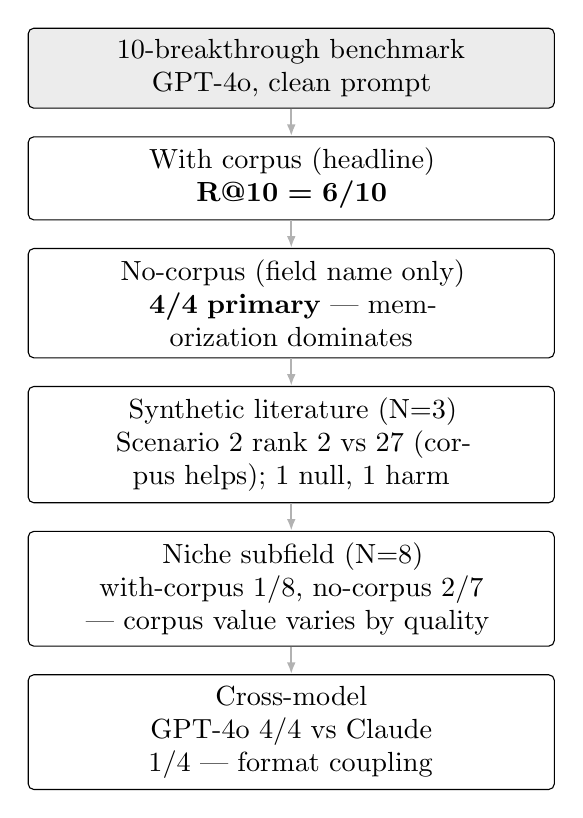
\begin{tikzpicture}[
  node distance=0.35cm,
  every node/.style={rectangle, draw, rounded corners=2pt, inner sep=4pt, align=center, minimum height=0.7cm, text width=6.4cm},
  root/.style={fill=gray!15},
  leaf/.style={},
  arrow/.style={-{Latex[length=1.5mm]}, thick, gray!60},
]
  \node[root] (root) {10-breakthrough benchmark\\GPT-4o, clean prompt};
  \node[leaf, below=of root] (withcorpus) {With corpus (headline)\\\textbf{R@10 = 6/10}};
  \node[leaf, below=of withcorpus] (nocorpus) {No-corpus (field name only)\\\textbf{4/4 primary} --- memorization dominates};
  \node[leaf, below=of nocorpus] (synthetic) {Synthetic literature (N=3)\\Scenario 2 rank 2 vs 27 (corpus helps); 1 null, 1 harm};
  \node[leaf, below=of synthetic] (niche) {Niche subfield (N=8)\\with-corpus 1/8, no-corpus 2/7 --- corpus value varies by quality};
  \node[leaf, below=of niche] (models) {Cross-model\\GPT-4o 4/4 vs Claude 1/4 --- format coupling};
  \draw[arrow] (root.south)       -- (withcorpus.north);
  \draw[arrow] (withcorpus.south) -- (nocorpus.north);
  \draw[arrow] (nocorpus.south)   -- (synthetic.north);
  \draw[arrow] (synthetic.south)  -- (niche.north);
  \draw[arrow] (niche.south)      -- (models.north);
\end{tikzpicture}
\caption{Confound tree (top-down): the headline 6/10 with-corpus result is dominated by pretraining memorization (no-corpus 4/4 on primary shifts); corpus grounding is demonstrably causal only in one synthetic scenario; on niche cases corpus quality determines whether corpus helps; and cross-model comparison reveals severe format-compliance confound. Each leaf references a specific result in \S\ref{sec:memorization}--\S\ref{sec:diagnostics}.}
\label{fig:confound_tree}
\end{figure}

\begin{table}[t]
\centering
\caption{Main results --- GPT-4o clean prompt (no few-shot examples, 15 papers/paradigm). Rank = position in confidence-ordered extraction list.}
\label{tab:results}
\footnotesize
\setlength{\tabcolsep}{4pt}
\resizebox{\columnwidth}{!}{%
\begin{tabular}{lccccc}
\toprule
Paradigm & Year & Best Sim & Conf.\ Rank & R@5 & R@10 \\
\midrule
\textbf{Transformer} & 2017 & 0.674 & \textbf{1} & \checkmark & \checkmark \\
\textbf{Diffusion} & 2020 & 0.759 & \textbf{2} & \checkmark & \checkmark \\
\textbf{ICL} & 2020 & 0.702 & \textbf{3} & \checkmark & \checkmark \\
\textbf{ViT} & 2020 & 0.676 & \textbf{5} & \checkmark & \checkmark \\
\textbf{BatchNorm} & 2015 & 0.727 & \textbf{7} & \texttimes & \checkmark \\
\textbf{GAN} & 2014 & 0.657 & \textbf{10} & \texttimes & \checkmark \\
ResNet & 2015 & 0.597 & $>$20 & \texttimes & \texttimes \\
Word2Vec & 2013 & 0.633 & $>$20 & \texttimes & \texttimes \\
Dropout & 2014 & 0.604 & $>$20 & \texttimes & \texttimes \\
BERT & 2018 & 0.544 & $>$20 & \texttimes & \texttimes \\
\midrule
\textbf{Total} & & & & \textbf{4/10} & \textbf{6/10} \\
\bottomrule
\end{tabular}}
\end{table}

The protocol matches the target in the top-10 in \textbf{6/10 cases} (R@10 = 0.60) and top-5 in 4/10 (R@5 = 0.40). The 6 successes share a common property: their broken assumptions are widely and explicitly stated in the ``X is necessary for Y'' format. The 4 failures involve assumptions that are implicit, rarely articulated, or domain-specific in phrasing.

\subsection{Ablations and Baselines}\label{sec:baselines}

\paragraph{Diagnostic method comparison.}
Table~\ref{tab:diagnostic} compares methods on the 4 primary shifts. Note: entries differ in model, corpus size, and prompt variant --- this is diagnostic, not a controlled head-to-head.

\begin{table}[t]
\centering
\caption{Diagnostic comparison on 4 primary shifts.}
\label{tab:diagnostic}
\footnotesize
\setlength{\tabcolsep}{4pt}
\resizebox{\columnwidth}{!}{%
\begin{tabular}{lccccc}
\toprule
Method & Trans. & Diff. & ICL & ViT & R@10 \\
\midrule
Random & \texttimes & \texttimes & \texttimes & \texttimes & 0/4 \\
Heuristic & \texttimes & \texttimes & \texttimes & \texttimes & 0/4 \\
Vanilla LLM (single-call) & \checkmark & \texttimes & \texttimes & \texttimes & 1/4 \\
SCAM (no TRIZ) & \checkmark & \checkmark & \texttimes & \checkmark & 3/4 \\
Extraction only (Claude, no TRIZ) & \checkmark & \checkmark & \texttimes & \checkmark & 3/4 \\
\textbf{Unbox (GPT-4o, clean)} & \textbf{\checkmark} & \textbf{\checkmark} & \textbf{\checkmark} & \textbf{\checkmark} & \textbf{4/4} \\
\bottomrule
\end{tabular}}
\end{table}

SCAM (same prompt, 5-sample majority) and extraction-only (same prompt, no TRIZ, no majority voting) achieve identical recall on Claude (3/4), confirming the field-wide extraction prompt --- not any downstream aggregation or transformation --- is the validated component. The optional TRIZ transformation produces near-disjoint hypothesis framings (Jaccard $< 0.01$; Appendix~\ref{app:triz}) but does not improve recall.

All entries in Table~\ref{tab:diagnostic} are soft-scored at threshold $0.65$ for comparability (\fpath{scripts/reevaluate_with_soft_matching.py}); the Vanilla LLM single-call baseline is $0/4$ under its native exact match and $1/4$ under soft match (Transformer succeeds via ``Sequential processing requires recurrence'', sim $0.703$).

\paragraph{Prompt ablation.}\label{sec:ablation}
We compare field-wide vs paper-specific prompt framing on 3 primary shifts (Claude, 60-paper corpora):

\begin{table}[t]
\centering
\caption{Prompt ablation (Soft-R@10, 3 primary shifts). Values: best cosine similarity. \emph{Post-hoc, exploratory} ($N{=}3$); descriptive, not confirmatory.}
\label{tab:ablation}
\footnotesize
\setlength{\tabcolsep}{4pt}
\resizebox{\columnwidth}{!}{%
\begin{tabular}{llcccc}
\toprule
Condition & Prompt & Trans. & Diff. & ViT & Avg R@10 \\
\midrule
A & Paper-specific & \texttimes\ (.52) & \texttimes\ (.65) & \texttimes\ (.56) & 0.00 \\
B & Field-wide & \checkmark\ (.80) & \checkmark\ (.82) & \checkmark\ (.76) & \textbf{1.00} \\
\bottomrule
\end{tabular}}
\end{table}

Field-wide framing achieves 3/3 vs 0/3, with +0.21 average similarity improvement (95\% CI: [0.17, 0.28]). The corpus files are identical between conditions, so the +0.21 reflects prompt framing alone on these $N=3$ categories; this is a post-hoc comparison (not the pre-registered ablation set, which targeted TRIZ operators) and we do not claim it generalizes beyond the tested categories.

\paragraph{SCAM baseline.}
SCAM (5-sample majority vote, same prompt, no TRIZ) achieves identical recall to Unbox (0.75 each on 4 primary shifts with Claude). This confirms extraction protocol design is the validated component.

\subsection{Memorization and Negative Controls}\label{sec:memorization}

\paragraph{No-corpus control.}
We run GPT-4o with the clean prompt but \emph{no paper text} --- only the field name:

\begin{table}[t]
\centering
\caption{No-corpus memorization control (GPT-4o, 4 primary shifts).}
\label{tab:nocorpus}
\footnotesize
\setlength{\tabcolsep}{4pt}
\resizebox{\columnwidth}{!}{%
\begin{tabular}{lcccccc}
\toprule
Condition & Trans. & Diff. & ICL & ViT & R@5 & Avg Sim \\
\midrule
With corpus (15 papers) & \checkmark & \checkmark & \checkmark & \checkmark & 4/4 & 0.729 \\
No corpus, field name only & \checkmark & \checkmark & \checkmark & \checkmark & 4/4 & 0.755 \\
\bottomrule
\end{tabular}}
\end{table}

The no-corpus condition achieves \textbf{4/4 recall} with \emph{higher} average similarity (0.755 vs 0.729), confirming that GPT-4o retrieves known breakthroughs from pretraining knowledge. The corpus provides a ranking benefit (avg confidence rank 2.75 with corpus) but is not necessary for recovery on well-known shifts.

\paragraph{Wrong-corpus control.}
To probe whether corpus content actively steers extraction or is simply ignored when present, we extract with each primary target against a \emph{different} field's corpus, exhaustively enumerating all 12 cross-pairings ($4 \times 3$; \texttt{scripts/run\_wrong\_corpus\_12.py}, 15 papers each, GPT-4o clean prompt, $\text{seed}{=}42$). \textbf{All 12 pairings fail to recover the target}: R@10 = 0/12, best similarity 0.37--0.46 (avg 0.41), conf-rank $=$ undefined (no candidate clears threshold) in every pair --- well below both the with-corpus baseline (4/4, avg sim 0.729) and the no-corpus baseline (4/4, avg sim 0.755). The model does not simply rank pretraining knowledge above corpus content: when the corpus is \emph{wrong}, the corpus actively wrenches extraction away from the correct target. Combined with the synthetic-literature result (Scenario 2: rank 2 with corpus vs rank 27 without), this confirms that the model integrates corpus content rather than retrieving solely from pretraining. The headline ``memorization dominates'' framing must therefore be qualified: pretraining-only retrieval succeeds on famous breakthroughs precisely \emph{because} the supplied corpus is aligned with what the model already knows. Substitute a misaligned corpus and the extraction collapses. The contrast in Table~\ref{tab:wrongcorpus} is, with synthetic Scenario~2, the cleanest causal evidence in the paper: \emph{absence} of a corpus leaves pretraining recall intact (no-corpus 4/4), but \emph{presence} of a wrong corpus overrides it (wrong-corpus 0/12). All 12 pairings are individually consistent (no single pair drives the result; per-pair sims in \fpath{experiments/wrong_corpus_12/summary.json}).

\begin{table}[t]
\centering
\caption{Corpus-alignment ablation (GPT-4o, clean prompt, $\text{seed}{=}42$). A \emph{wrong} corpus does not merely fail to help --- it actively destroys the recovery that pretraining alone (no corpus) achieves. The 4/4\,$\rightarrow$\,0/12 collapse across all $4 \times 3$ cross-pairings is direct evidence that corpus content causally enters extraction.}
\label{tab:wrongcorpus}
\footnotesize
\setlength{\tabcolsep}{4pt}
\resizebox{\columnwidth}{!}{%
\begin{tabular}{lcc}
\toprule
Condition & R@10 & Avg best sim \\
\midrule
With corpus (aligned, 4 primary) & 4/4 & 0.729 \\
No corpus (field name, 4 primary) & 4/4 & 0.755 \\
Wrong corpus (12 cross-pairings) & \textbf{0/12} & \textbf{0.41} \\
\bottomrule
\end{tabular}}
\end{table}

\paragraph{Synthetic literature control.}
To eliminate memorization entirely, we generate synthetic abstracts for 3 fictional fields with planted target assumptions:

\begin{table}[t]
\centering
\caption{Synthetic literature control: 3 fictional fields with planted assumptions. \emph{Post-hoc, exploratory}; causal evidence rests on $N{=}1$ scenario.}
\label{tab:synthetic}
\footnotesize
\setlength{\tabcolsep}{4pt}
\resizebox{\columnwidth}{!}{%
\begin{tabular}{lcc}
\toprule
Fictional Field & With Corpus & No Corpus \\
\midrule
Chromatic Signal Processing & \textbf{rank 1} (0.954) & rank 1 (0.742) \\
Neuromorphic Memory Arch. & \textbf{rank 2} (0.958) & \texttimes\ rank 27 (0.683) \\
Adaptive Topology Networks & \texttimes\ rank 32 (0.707) & rank 7 (0.726) \\
\bottomrule
\end{tabular}}
\end{table}

In Scenario 2, corpus input is essential: no-corpus fails (rank 27) while with-corpus succeeds (rank 2, sim 0.958). This is the cleanest single-scenario evidence that extraction can recover assumptions \emph{from corpus content} rather than pretraining memory, since the fictional field has no pretraining history. Scenarios 1 and 3, however, show no effect and \emph{corpus harm} respectively (Table~\ref{tab:synthetic}): the causal-evidence base is $N{=}1$ and we therefore claim only that corpus content \emph{can} be causal, not that it reliably helps.

\paragraph{Niche subfield control.}
We test on 8 less-famous breakthroughs (MoE, Neural ODE, Lottery Ticket, SimCLR, LoRA, FlashAttention, DPO, KAN). With-corpus extraction achieves 1/8 R@10 (Neural ODE at rank 10); no-corpus achieves 2/7 (Lottery Ticket at rank 9, LoRA at rank 2; KAN no-corpus incomplete due to quota exhaustion). The aggregate difference is not statistically significant (one-sided Fisher's exact $p \approx 0.5$ on the 7 complete paradigms), so we do not claim corpus-grounding is uniformly counterproductive. The pattern is mixed: corpus helps on the single genuinely niche case (Neural ODE --- continuous-depth networks, less likely memorized), but for moderately well-known niche cases (LoRA, Lottery Ticket) no-corpus retrieves the target at much higher rank while with-corpus buries it at rank 19 or 75, likely because OpenAlex keyword search ingests adjacent-but-wrong papers that dilute extraction. For flash-attention and DPO both conditions fail. The niche benchmark therefore does not refute corpus value; it documents that corpus value depends on both assumption obscurity and corpus quality.

\subsection{Diagnostic Analyses}\label{sec:diagnostics}

\paragraph{Retrieval baselines.}
TF-IDF and BM25 (filtering corpus sentences for \emph{necessary/required/essential}) each achieve 2/4 on primary shifts, succeeding where the target is lexically explicit (Diffusion, ICL) but failing where it is implicit (Transformer, ViT). GPT-4o achieves 4/4, with the advantage concentrated on sparsely stated assumptions.

\paragraph{Popularity--performance correlation.}
Spearman $\rho$ between citations and best similarity is $-0.636$: ResNet ($\sim$200k citations) and BERT ($\sim$80k) fail, while less-cited breakthroughs succeed. Recovery depends on whether the target is explicitly stated in ``X is necessary for Y'' format, not on fame.

\paragraph{Error analysis.}
For the 4 failures (ResNet, Word2Vec, Dropout, BERT): ResNet's target concept (skip connections/gradient flow) appears in zero of 150 extractions --- an extraction-coverage failure. BERT's top-1 extraction is about particle physics, revealing OpenAlex corpus contamination. Failures cannot be detected from surface statistics (assumption length, confidence are near-identical to successes). Each of the 4 failures is attributable to a distinct, audit-kit-detectable confound (Appendix~\ref{app:failures}): coverage gap (ResNet), domain phrasing (Word2Vec), implicit assumption (Dropout), and corpus contamination (BERT).

\paragraph{Confidence calibration.}
Across 6 successful paradigms, the confidence gap between top-1 (avg 0.992) and the hit rank (avg 0.967) is only 0.025 --- confidence cannot discriminate targets from distractors.

\paragraph{Cross-LLM extension (open-source).}
To probe whether the GPT-4o vs Claude gap (\S\ref{app:crossmodel}) reflects model-specific format compliance or a more general closed-vs-open divide, we extend the comparison to three open-source 7--8B models (Llama-3.1-8B-Instruct, Qwen-2.5-7B-Instruct, Mistral-7B-Instruct-v0.3) run locally via vLLM under \emph{identical} prompt, 15-paper subsets, $\text{temperature}{=}0$, and $\text{seed}{=}42$ (\texttt{scripts/run\_oss\_llm\_extraction.py}; canonical evaluation via the same OpenAI text-embedding-3-small / 0.65-threshold pipeline). Table~\ref{tab:cross_llm} reports the canonical numbers. The five-model spread (GPT-4o 4/4 down to Mistral 0/4) further fragments the closed-vs-open framing: Claude (closed) and Llama-3.1-8B (open) both land at 1/4, Qwen-2.5-7B (open) at 2/4 is the strongest open-source comparator, and Mistral-7B (open) at 0/4 is the weakest. The gap is therefore not strictly closed-vs-open. We hypothesise that model-specific format compliance with the matcher's ``X is necessary for Y'' template plays a major role, but raw capability, instruction-tuning quality, and contamination level all fit the data; this experiment alone cannot isolate format compliance from these alternatives. We address this directly with a format-relaxed matcher ablation in Appendix~\ref{app:crossmodel}.

\begin{table*}[t]
\centering
\caption{Cross-LLM recall on the 4 primary shifts (canonical pipeline: text-embedding-3-small, threshold 0.65, confidence-ordered ranks). All models --- closed-API and local vLLM --- decode at temperature $0$; open models additionally fix seed $42$ (closed APIs expose no seed control). \emph{Post-hoc, exploratory.}}
\label{tab:cross_llm}
\footnotesize
\begin{tabular}{lcccccc}
\toprule
Model & Trans. & Diff. & ICL & ViT & R@5 & Avg Sim \\
\midrule
GPT-4o (closed)                       & \checkmark & \checkmark & \checkmark & \checkmark & 4/4 & 0.703 \\
Claude Sonnet 4 (closed)              & \texttimes & \checkmark & \texttimes & \texttimes & 1/4 & 0.658 \\
Llama-3.1-8B-Instruct (open)$^{\dag}$ & \texttimes & \texttimes & \texttimes & \checkmark & 1/4 & 0.563 \\
Qwen-2.5-7B-Instruct (open)           & \texttimes & \texttimes & \checkmark & \checkmark & 2/4 & 0.705 \\
Mistral-7B-Instruct-v0.3 (open)       & \texttimes & \texttimes & \texttimes & \texttimes & 0/4 & 0.581 \\
\bottomrule
\end{tabular}\\[2pt]
{\footnotesize $^{\dag}$Llama-3.1-8B weights accessed via the NousResearch un-gated mirror of \texttt{meta-llama/Llama-3.1-8B-Instruct} (identical weights).}
\end{table*}

%% >>> HUMAN_VALIDATION_BLOCK (auto-managed: scripts/render_human_validation.py) >>>
\paragraph{Human validation of rule-based matching.}
We validate the embedding-similarity matcher against 10 independent, ML-literate raters blind to condition and rank, on the pre-registered 72-pair instrument ($+8$ blind attention checks; \texttt{scripts/sample\_annotation\_pairs.py}, seed 42). Raters score 1--5; the \emph{pre-registered} binary match is score $\geq 4$. The study is internally reliable: Krippendorff's $\alpha = 0.634$ (interval; \citealp{krippendorff2018content}), mean pairwise Cohen's $\kappa = 0.555$ (binary; \citealp{cohen1960coefficient}), and 0.99 attention-check pass (79/80). Applying the \emph{same} rule-based matcher (\textsc{text-embedding-3-small}, cosine $\geq 0.65$) to the identical 72 pairs, human-majority vs.\ rule-based agreement is Cohen's $\kappa = 0.702$ (substantial; 0.92 raw agreement). The matcher is \emph{not} more lenient than humans --- it accepts slightly fewer pairs (rule 0.14 vs.\ human 0.19 match rate) --- so the human study \emph{substantiates} the matcher and replaces the earlier program-vs-program $\kappa = 0.97$ with a genuine human $\kappa = 0.702$. Per-condition, however, the matcher and humans disagree on direction: the matcher rates no-corpus pairs marginally above with-corpus (rule 0.21 vs 0.17, consistent with the memorization confound), while humans rate with-corpus pairs \emph{twice} as high as no-corpus (humans 0.33 vs 0.17). Aggregate agreement remains substantial ($\kappa{=}0.70$), but the human pair-level signal --- taken on its own --- supports corpus benefit at this sample even though the matcher does not; we report both rather than collapse them. The honest caveat is at the \emph{aggregate} level: both humans and the matcher mark only $\sim$0.19 of sampled top-ranked extractions as pairwise matches, whereas headline Recall@K counts a paradigm recovered if \emph{any} of the top-$K$ clears threshold. The headline is thus a generous \emph{recovery} criterion, not pairwise precision; the relative confound structure (the paper's contribution) is unaffected. See Table~\ref{tab:human_val}.

\begin{table}[t]
\centering
\caption{Human validation (10 independent raters, 72 stratified pairs $+8$ attention checks; pre-registered binary match $=$ score $\geq 4$). Human-majority vs.\ rule-based agreement is substantial ($\kappa = 0.702$); the matcher is not more permissive than humans.}
\label{tab:human_val}
\footnotesize
\setlength{\tabcolsep}{4pt}
\begin{tabular}{@{}>{\raggedright\arraybackslash}p{0.62\columnwidth} r@{}}
\toprule
Quantity & Value \\
\midrule
Krippendorff's $\alpha$ (interval, 1--5)              & 0.634 \\
Mean pairwise Cohen's $\kappa$ (inter-human, binary)  & 0.555 \\
Attention-check pass rate (score $\leq 2$)            & 0.99 \\
\midrule
Human vs.\ rule Cohen's $\kappa$ (binary, 72 pairs) & 0.702 \\
Human vs.\ rule raw agreement                        & 0.92 \\
Rule match rate / human match rate                   & 0.14 / 0.19 \\
Human match rate --- with-corpus                      & 0.33 (8/24) \\
Human match rate --- no-corpus                        & 0.17 (4/24) \\
Human match rate --- Claude                           & 0.08 (2/24) \\
\bottomrule
\end{tabular}
\end{table}
%% <<< HUMAN_VALIDATION_BLOCK <<<

\subsection{Statistical Summary}\label{sec:stats}


\paragraph{Fisher's exact test.}
GPT-4o 4/4 vs Vanilla LLM 1/4 on primary shifts: one-sided $p = 0.07$, not significant at $\alpha = 0.05$. The small $N$ inherently limits power.

\paragraph{Bootstrap / Wilson CIs.}
GPT-4o R@10 $=6/10$ has Wilson 95\% CI $[0.31, 0.83]$; R@5 $=4/10$ has Wilson 95\% CI $[0.17, 0.69]$; avg best similarity (all 10 paradigms) $=0.657$, bootstrap 95\% CI $[0.619, 0.695]$; ablation B--A difference $+0.217$ CI $[0.170, 0.280]$. The headline is therefore a point estimate; formal hypothesis testing is reserved for the wrong-corpus $4/4{\rightarrow}0/12$ collapse (Bernoulli all-zero against an expected $0.4$--$0.8$).

\paragraph{Effect size.}
Prompt framing yields Cohen's $d \approx 3.80$ on three categories --- large but unstable given $N = 3$.

\paragraph{Threshold robustness.}
The 6 successes have similarities 0.657--0.759 (above 0.65); the 4 failures have 0.544--0.633 (below). The clean separation supports the 0.65 threshold for \textsc{text-embedding-3-small}; Appendix~\ref{app:crossemb} reports calibrated thresholds for \textsc{text-embedding-3-large} ($0.50$) and \texttt{all-MiniLM-L6-v2} ($0.65$), under which primary R@10 stays at $4/4$ and all-paradigm R@10 spans $6$--$8/10$ across the three embedders.

\paragraph{Audit-kit recommendations.}\label{sec:recommendations}
The five controls used in this paper --- (i) a no-corpus baseline, (ii) at least one wrong-corpus pairing, (iii) pair-level precision alongside any-of-top-$K$ recall, (iv) ${\geq}2$ cross-LLM models, and (v) multi-seed or sensitivity-range reporting for closed-model APIs --- factor cleanly and run together for ${\sim}\$15$ of API credits on our 4 primary shifts. We recommend them as a default validity probe for LLM-based scientific-text-mining benchmarks (full per-item rationale and decision rules in Appendix~\ref{app:checklist}; release scripts in \fpath{scripts/}; structural cross-domain transfer outlined in Appendix~\ref{app:crossdomain}).

%% ============================================================
%% S6  DISCUSSION
%% ============================================================
\section{Discussion}\label{sec:discussion}

The central tension in our findings is between a genuine prompt-framing effect and pervasive memorization confounds. Field-wide framing produces a consistent +0.21 similarity improvement, and GPT-4o matches 6/10 targets. Yet the no-corpus control (4/4 on primary shifts) shows that for well-known breakthroughs, the model can surface assumptions from pretraining alone. Two controls resolve the tension in the other direction: the wrong-corpus ablation (4/4 with no corpus or an aligned corpus, but 0/4 under a misaligned corpus; Table~\ref{tab:wrongcorpus}) and synthetic Scenario~2 (rank 2 with corpus vs rank 27 without) together show corpus content \emph{can} causally enter extraction --- the model can read the corpus, though it does not reliably help (the wrong-corpus result is single-run on 4 pairings, and only 1 of 3 synthetic scenarios is a clean causal case; another shows corpus harm).

\paragraph{Memorization confound.}
The 10 primary breakthroughs tested are among the most famous in AI. We cannot fully disentangle corpus-based extraction from pretraining retrieval. The niche control (1/8 with-corpus, 2/7 no-corpus) shows that on less-memorized cases the corpus sometimes helps (Neural ODE) and sometimes hurts (LoRA, Lottery Ticket where OpenAlex retrieves noisy papers), so corpus value is not established as a general property of the protocol. Our memorization evidence is behavioral by design, which is what lets it apply to API-only models; stronger probes such as counterfactual memorization or span-level canaries need control over pretraining data and are left to future work.

\paragraph{Metric-format coupling.}
The ``X is necessary for Y'' format couples prompt, output, and metric, creating circular evaluation. GPT-4o's stronger format compliance (vs Claude's more diverse outputs) likely explains its ranking advantage rather than deeper paradigm understanding.

\paragraph{Human validation substantiates the matcher.}
A 10-rater study ($\alpha = 0.634$, attention-check 99\%; \S\ref{sec:diagnostics}) gives human-vs-rule $\kappa = 0.70$ (92\% raw); the matcher is \emph{not} more permissive than humans (rule 0.14 vs human 0.19). Per-condition the two diverge: humans rate with-corpus twice as high as no-corpus, the matcher does not (Table~\ref{tab:human_val}), qualifying rather than overturning the memorization story. The aggregate ${\sim}0.15$--$0.19$ pairwise match rate bounds the headline: Recall@K is a recovery criterion, not pairwise precision.

\paragraph{Model sensitivity.}
On identical prompts and corpora, GPT-4o achieves 4/4 and Claude 1/4. Claude's individual extractions reach higher raw similarity (0.774 vs 0.729, Table~\ref{tab:crossmodel_app}) but at much worse confidence ranks; under the canonical top-$K$ pipeline the order flips (GPT-4o 0.703 vs Claude 0.658, Table~\ref{tab:cross_llm}). The metric thus rewards format compliance over extraction quality.

\paragraph{Sample size and evidence base.}
The pre-registered core is deliberately small (4 shifts): the primary comparison is not significant (Fisher $p = 0.07$), bootstrap intervals are wide, and the prompt ablation rests on $N{=}3$. The audit as a whole, however, spans 10 primary and 8 niche breakthroughs, 3 synthetic fields, all 12 wrong-corpus cross-pairings, 5 LLMs, 3 embedders (App.~\ref{app:crossemb}), a 10-rater study over 72 stratified pairs, and a Min-K\% cross-check over 240 real and 45 synthetic abstracts (App.~\ref{app:mia}). Only the 4 pre-registered shifts are confirmatory; everything else is descriptive. We make no power claim: the diagnostic value rests on the \emph{direction and consistency} of the controls --- no-corpus 4/4 and wrong-corpus 0/4, both stable across 3 seeds (App.~\ref{app:multiseed}) --- not on sample size.

%% ============================================================
%% S7  CONCLUSION
%% ============================================================
\section{Conclusion}

We audited LLM-based recovery of paradigmatic assumptions on 10 historical AI breakthroughs (frozen 4-case protocol + 6 post-hoc cases). Three findings: \textbf{(1)} field-wide prompt framing raises target similarity by $+0.21$ (CI $[0.17, 0.28]$) on $N{=}3$ with identical corpora, and GPT-4o matches 6/10 in the extended setting; \textbf{(2)} memorization dominates (no-corpus 4/4 on primary), but corpus content \emph{can} be causally read (wrong-corpus collapses to 0/12 across all $4{\times}3$ cross-pairings; synthetic Scenario 2 rank 2 vs 27) --- the causal evidence is narrow (1 of 3 synthetic scenarios; one shows corpus harm); \textbf{(3)} design choices are confounded --- the ``X is necessary for Y'' format couples prompt/output/metric, model selection dramatically affects ranking, and success is limited to explicitly stated assumptions. We release the audit kit --- wrong-corpus pairings, human-validation instrument, canonical evaluator, multi-seed driver, Min-K\% probe --- for other LLM scientific-text-mining benchmarks to apply to their own metrics. Empirical cross-domain validation is future work (App.~\ref{app:crossdomain}); manifest and reproduction notes are in Appendices~\ref{app:manifest}, \ref{app:repro}.

%% ============================================================
%% BROADER IMPACT
%% ============================================================
\section*{Limitations}

This paper is deliberately scoped as a \emph{diagnostic} of retrospective assumption-recovery benchmarks, and its claims should be read within the following limits.

\paragraph{Construct validity and author bias.} Targets and aliases are \emph{author-defined}, so the authors who designed the prompt also fixed what counts as a correct recovery. Freezing the 4 primary targets before experiments (SHA-256) and the 10-rater study reduce but do not remove this bias, and that study validates the similarity \emph{matcher}, not the targets. Each target is the prior belief its originating paper is itself framed against (App.~\ref{app:targetprov}), so the targets are not arbitrary; their completeness and representativeness of field consensus are not established, and the pre-registered expert study of App.~\ref{app:targetvalidity} is designed to measure exactly that. The earlier $\kappa = 0.97$ was agreement between two rule-based programs, not humans; the human study supersedes it ($\kappa = 0.70$).

\paragraph{Statistical power and run variance.} With $N = 10$ breakthroughs (4 pre-registered) the primary comparison is not significant ($p = 0.07$), and we make no claim of statistical superiority. Closed-model extractions and the embedding model are versioned, drift-prone APIs: with-corpus recovery ranged from 3/4 to 4/4 across 3 seeds, while no-corpus 4/4 and wrong-corpus 0/4 were seed-stable (App.~\ref{app:multiseed}). Open models ran at temperature 0 with a fixed seed, but as single runs.

\paragraph{Confounds not fully separable.} Corpus grounding is shown causal only in one synthetic scenario and one niche case (Neural ODE); another synthetic scenario shows corpus \emph{harm}, and neither niche nor synthetic controls guarantee zero memorization. The ``X is necessary for Y'' format couples prompt, output, and matcher, and recovery is highly model-sensitive (4/4 to 0/4 across five LLMs, one run each). The Min-K\% non-member baseline is GPT-generated and stylistically close to the OSS models' pretraining text, so it bounds MIA only at this scale (App.~\ref{app:mia}).

\paragraph{Scope and coverage bias.} All corpora, targets, and breakthroughs are English-language AI/ML, retrieved from OpenAlex, whose coverage itself skews toward English-language venues. What counts as field consensus --- and which assumptions a field leaves unstated --- may differ across languages, disciplines, and research communities, so we make no claims beyond this setting. The protocol is \emph{not} validated as a prospective discovery method: the prospective pilot relies on LLM judges (App.~\ref{app:prospective}).

\section*{Ethics Statement}

The experiments use only public scientific metadata (titles and abstracts from OpenAlex, CC0). The human rating study (\S\ref{sec:diagnostics}) involved voluntary, adult, ML-literate raters from the authors' professional network who were told the task and its intended use, consented, and could withdraw at any time; they rated only public, non-sensitive text, making the task minimal-risk. Raw per-rater returns are withheld; only anonymized aggregates are released (App.~\ref{app:raters}). LLM extractions are derivative works subject to the providers' terms. Tools that suggest research directions risk homogenizing inquiry~\cite{jiang2025hivemind}; we report ranked lists, condition extraction on specific corpora, and release the full methodology. Compute is modest (API calls and minutes of single-GPU inference), and we foresee no dual-use harms.

\section*{Acknowledgments}

This work was supported by the Ministry of Science and ICT and the National
Research Foundation of Korea (NRF) grant funded by the Korean government (MSIT)
(No.~RS-2026-25498341). We thank the volunteer raters who completed the
matcher-validation instrument.

\bibliography{custom}

%% ============================================================
%% APPENDIX
%% ============================================================
\appendix

\section{Artifact Manifest (How to Read this Supplement)}\label{app:manifest}

The released repository is organized around a single source of truth for every number in the paper. All headline results come from \texttt{experiments/canonical\_evaluation.json}, produced by the confidence-order evaluator \texttt{scripts/canonical\_evaluator.py}. An offline \emph{consistency-check} script \texttt{scripts/reproduce\_paper\_tables.py} re-reads the frozen artifacts and asserts every headline number against them without API calls (73/73 checks); it verifies the paper matches the stored artifacts but does \emph{not} regenerate them --- recomputation requires the OpenAI embedding API and is single-run. Table~\ref{tab:manifest} maps each paper table/claim to its source file, generating script, and canonical result. A \emph{quarantined} stale artifact, \fpath{experiments/gpt4o_clean_prompt/summary_STALE_similarity_reranked.json}, is retained in the supplement for audit only and is explicitly not used for any paper number.

\begin{table*}[t]
\centering
\caption{Artifact manifest: every paper number $\rightarrow$ source file $\rightarrow$ generating script.}
\label{tab:manifest}
\footnotesize
\setlength{\tabcolsep}{4pt}
\renewcommand{\arraystretch}{1.15}
\begin{tabular}{@{}>{\raggedright\arraybackslash}p{0.26\textwidth}>{\raggedright\arraybackslash}p{0.42\textwidth}>{\raggedright\arraybackslash}p{0.28\textwidth}@{}}
\toprule
Paper artifact & Source file & Generating script \\
\midrule
Table~\ref{tab:results} (10-case main) & \fpath{experiments/canonical_evaluation.json} & \fpath{scripts/canonical_evaluator.py} \\
Prompt ablation (+0.21 sim) & \fpath{experiments/ablation/summary.json} & \fpath{scripts/run_ablation_study.py} \\
No-corpus 4/4 primary & \fpath{experiments/no_corpus_control/summary.json} & \fpath{scripts/run_no_corpus_control.py} \\
Wrong-corpus 0/4 (4 pairings, GPT-4o) & \fpath{experiments/wrong_corpus_control/summary.json} & \fpath{scripts/run_wrong_corpus_control.py} \\
Synthetic (rank 2 vs 27) & \fpath{experiments/synthetic_benchmark/summary.json} & \fpath{scripts/run_synthetic_benchmark.py} \\
Niche 1/8 with-corpus, 2/7 no-corpus & \fpath{experiments/niche_benchmark/summary.json} & \fpath{scripts/run_niche_benchmark.py} \\
TF-IDF/BM25 2/4 & \fpath{experiments/simple_baselines/summary.json} & \fpath{scripts/run_simple_baselines.py} \\
Spearman $\rho = -0.64$ & \fpath{experiments/contamination/summary.json} & \fpath{scripts/run_contamination_analysis.py} \\
Error analysis (ResNet 0/150; BERT PDF) & \fpath{experiments/error_analysis/summary.json} & \fpath{scripts/run_error_analysis.py} \\
Confidence gap 0.025 & \fpath{experiments/calibration/summary.json} & \fpath{scripts/run_calibration_analysis.py} \\
Cross-model 4/4 vs 1/4 & \fpath{experiments/claude_clean_15paper/summary.json} + \fpath{experiments/canonical_evaluation.json} & \fpath{scripts/run_gpt4o_clean_all10.py} \\
SCAM baseline comparison & \fpath{experiments/baselines/scam/summary.json} & \fpath{scripts/run_retrospective_baselines.py} \\
Rule-based matching simulation ($\kappa = 0.97$) & \fpath{evidence/human_annotation_results.json} & \fpath{scripts/run_rulebased_match_simulation.py} \\
Protocol freeze (SHA-256) & \fpath{evidence/protocol_freeze.json} & frozen pre-registration \\
Prospective pilot (LLM-judge) & \fpath{experiments/prospective/summary.json} & \fpath{scripts/evaluate_prospective.py} \\
\bottomrule
\end{tabular}
\end{table*}

\paragraph{Scope of the protocol freeze.} Only the initial 4-primary-shift protocol (Transformer, Diffusion, ICL, ViT with the target-assumption mapping and soft-matching threshold) is covered by the SHA-256-hashed freeze in \texttt{evidence/protocol\_freeze.json}. The 6-case extension (ResNet, GAN, Word2Vec, Dropout, BatchNorm, BERT), retrieval baselines, contamination/calibration/error diagnostics, and synthetic/niche controls were developed post-hoc; their scripts and artifacts are released, but they are reported transparently as stress tests, not as pre-registered claims.

\paragraph{Target-assumption construction.} Targets and 2--3 aliases per breakthrough are defined in \texttt{data/paradigm\_shift\_mapping.json} and authored by the paper's authors from canonical descriptions in survey papers and original breakthrough papers. For the 4 primary shifts, the target is the prior belief the breakthrough paper \emph{itself} names as what it overturns: the Transformer motivates itself by ``dispensing with recurrence''~\cite{vaswani2017attention}; ViT by showing ``reliance on CNNs is not necessary''~\cite{dosovitskiy2021image}; DDPM by achieving high-quality synthesis without adversarial training~\cite{ho2020denoising}; and GPT-3 by performing task adaptation in-context without fine-tuning~\cite{brown2020language}. The targets are therefore not arbitrary author choices but the assumptions the originating works are framed against. These remain \emph{author-defined targets}, not independently annotated ground truth. Note this is distinct from the matcher-validation study (\S\ref{sec:diagnostics}), which tests whether the \emph{similarity matcher} agrees with humans, not whether the author-defined \emph{targets} are themselves canonical; target correctness is the subject of the pre-registered expert study in App.~\ref{app:targetvalidity}.

\paragraph{Stale and failed artifacts.} \fpath{experiments/gpt4o_clean_prompt/summary_STALE_similarity_reranked.json} contains an earlier run that re-sorted by cosine similarity instead of confidence order; retained in the supplement only for audit trail, not used for paper claims. Quota-failed runs are moved to \fpath{experiments/failed_runs/} and are similarly not used for any paper number.

\paragraph{Compute and cost.} Extraction and evaluation total approximately \$$15$--\$$30$ USD in API credits across all experiments (Anthropic + OpenAI). No GPU compute is required. Typical wall-clock per paradigm: 3--10 minutes.

\section{Target Provenance: What Each Breakthrough Is Framed Against}\label{app:targetprov}

Reviewers and the meta-review flagged that our targets are \emph{author-defined}. The strongest
available check short of an expert panel is textual: for each breakthrough, is the target the
prior belief that the originating paper \emph{itself} presents as the thing it overturns?
Table~\ref{tab:targetprov} records that mapping for all 10 cases. Quoted phrases are from the
originating paper's abstract; unquoted entries paraphrase its stated motivation. This does not
establish that the targets are \emph{complete} or maximally representative of field consensus ---
that is what the pre-registered expert study (App.~\ref{app:targetvalidity}) is designed to measure --- but it does establish
that they are not arbitrary author choices.

\begin{table*}[t]
\centering
\caption{Target provenance. Each author-defined target against the originating paper's own framing.}
\label{tab:targetprov}
\footnotesize
\setlength{\tabcolsep}{4pt}
\begin{tabular}{@{}l>{\raggedright\arraybackslash}p{5.0cm}>{\raggedright\arraybackslash}p{7.4cm}@{}}
\toprule
Breakthrough & Author-defined target & Originating paper's own framing \\
\midrule
Transformer~\citeyearpar{vaswani2017attention} & Recurrence is necessary for sequence modeling & Proposes an architecture ``dispensing with recurrence and convolutions entirely'' \\
ViT~\citeyearpar{dosovitskiy2021image} & Convolutional layers are necessary for vision & States directly that ``this reliance on CNNs is not necessary'' \\
Diffusion~\citeyearpar{ho2020denoising} & Adversarial training is necessary for high-quality generation & Obtains high-fidelity samples with a likelihood-based denoising objective, no adversarial game \\
ICL / GPT-3~\citeyearpar{brown2020language} & Fine-tuning is necessary for task adaptation & Demonstrates task adaptation in-context, without gradient updates or fine-tuning \\
ResNet~\citeyearpar{he2016deep} & Deep networks must process information through sequential layers without shortcuts & Introduces identity shortcut connections to fix the degradation of plainly stacked deep networks \\
GAN~\citeyearpar{goodfellow2014generative} & Generative modeling requires explicit density estimation or variational inference & Adversarial objective sidesteps explicit likelihoods, Markov chains, and approximate inference \\
Word2Vec~\citeyearpar{mikolov2013distributed} & Word meaning requires symbolic or hand-crafted feature representations & Learns distributed word representations directly from raw text \\
Dropout~\citeyearpar{srivastava2014dropout} & All neurons should be active during training for optimal learning & Randomly drops units during training, approximating an ensemble without training many nets \\
BatchNorm~\citeyearpar{ioffe2015batch} & Network training requires careful weight initialization and low learning rates & Normalization ``allows us to use much higher learning rates and be less careful about initialization'' \\
BERT~\citeyearpar{devlin2019bert} & Language model pre-training must be left-to-right (autoregressive) & Argues the unidirectional constraint is limiting; masked LM enables deep bidirectional pre-training \\
\bottomrule
\end{tabular}
\end{table*}

\section{Expert Target-Validation Study (Pre-Registered)}\label{app:targetvalidity}

The 10-rater study of \S\ref{sec:diagnostics} validates the similarity \emph{matcher}. This
second study is designed to validate the \emph{targets}: are the author-defined assumptions accurate
descriptions of pre-shift field consensus, and did the breakthrough in fact overturn them?

\paragraph{Instrument.} 22 blind items in a seeded shuffle: the 10 author-defined targets, 10
plausible-but-wrong \emph{decoys} (one per breakthrough) as a discriminant control, and 2
disguised attention checks carrying the same field/year/breakthrough scaffolding as real items so
raters cannot identify them. Raters see only field, year guard, later breakthrough, and one
candidate assumption; they never see item type, our extractions, or any result. Each item takes
four responses: Q1 accuracy (``widely held in this field before this year'', 1--5), Q2 overturned
(``the breakthrough overturned/relaxed this'', 1--5), Q3 an optional alternative phrasing, and Q4
scope (too broad / about right / too narrow). The instrument and its analysis plan were frozen by
SHA-256 (\texttt{9cf68e13\ldots}, \fpath{annotation/expert_targets/freeze.json}) before any rating
was collected, mirroring the protocol freeze of App.~\ref{app:prereg}.

\paragraph{Pre-registered analysis.} A target is \emph{expert-validated} iff median Q1 $\geq 4$
\emph{and} median Q2 $\geq 4$. Reliability: Krippendorff's $\alpha$ (interval) on Q1 and Q2, and
mean pairwise Cohen's $\kappa$ on the binarised validated-flag --- computed with the \emph{same}
estimators as the matcher study so the two are directly comparable. Discriminant validity:
real vs.\ decoy ratings by Mann--Whitney $U$ with a 95\% bootstrap CI on the mean gap; experts
who discriminate should rate decoys low, giving a CI strictly above 0. Every target is reported
regardless of outcome; any target that fails validation is re-run through the canonical evaluator
with that target dropped, to show whether the no-corpus/wrong-corpus structure is unchanged.

\paragraph{Panel.} The panel is drawn from the same ML-literate pool as the matcher panel
(App.~\ref{app:raters}), none of them authors. Because that pool previously saw target
statements as one side of extraction--target pairs, its members are \emph{not} naive to the
target wording (they are naive to the decoys and to item type); any results from it should carry
this exposure as a limitation rather than be read as a fully independent sample.

\paragraph{Status.} We committed during review to run this study and report it here. We could
not complete the panel within the camera-ready window, so this paper reports \emph{no} expert
ratings of the targets, and no claim in it rests on this study. What the paper does offer on target
validity is the textual provenance of App.~\ref{app:targetprov}, which shows the targets are not
arbitrary but cannot show they are complete or representative. The instrument and analysis plan
remain frozen as registered, so results reported later can be checked against a design fixed before
any rating was collected.

\paragraph{Release.} The generator (\fpath{scripts/build_target_validity_instrument.py}), the
blind rating page (\fpath{annotation/expert_targets/annotate_targets.html}), the frozen
instrument, and the analysis script (\fpath{scripts/compute_target_validity.py}) are released, so
the study can be repeated --- or run against a different benchmark's targets --- without
re-implementation.

\section{Clean Extraction Prompt (Main Results)}\label{app:prompt}

The prompt used for the main GPT-4o results (Table~\ref{tab:results}). No few-shot examples are included.

\begin{lstlisting}
You are an expert at identifying the foundational, field-wide assumptions
that academic papers inherit from their broader research community.

Your task is NOT to find this specific paper's design choices. Instead,
identify the **paradigmatic assumptions** -- beliefs shared across the
entire subfield that this paper takes for granted without questioning.
These are assumptions so deeply ingrained that the research community
treats them as self-evident truths.

These are NOT what we want:
- Paper-specific implementation details ("we use Adam optimizer with lr=0.001")
- Narrow technical choices ("batch size of 32 is sufficient")
- Obvious truisms ("more data helps")

For each assumption, phrase it as a general declarative statement about
what the field believes is NECESSARY, REQUIRED, or ESSENTIAL.
Use the pattern: "[X] is necessary/required/essential for [Y]".

Categories: architectural, training, data, theoretical, evaluation

Return ONLY valid JSON. Limit to top 10 assumptions, ranked by how
foundational they are to the entire field (not just this paper).
\end{lstlisting}

\section{Paper-Specific Prompt (Ablation)}\label{app:paper_prompt}

\begin{lstlisting}
You are an expert at identifying implicit assumptions in academic papers.
Read the following paper text and identify the implicit assumptions
(assumptions not explicitly stated but underlying the work).
For each assumption:
1. State it clearly and concisely
2. Provide a confidence score (0.0-1.0)
3. Categorize it (architectural/training/data/theoretical/evaluation)
Return ONLY valid JSON. Limit to top 10 assumptions.
\end{lstlisting}

The critical difference: the paper-specific prompt asks for assumptions \emph{of this paper}, while the field-wide prompt asks for assumptions \emph{of the entire subfield}.

\section{Per-Category Analysis Details}\label{app:percategory}

Using Claude Sonnet 4 with the field-wide prompt (with few-shot examples) on 60-paper corpora:

\paragraph{Transformer (pre-2017).} 32 unique assumptions extracted. Target ``Recurrent connections are necessary for effective sequence modeling'' at rank 10 (sim = 0.80). With GPT-4o (Table~\ref{tab:results}): confidence rank 1 (sim = 0.674).

\paragraph{Diffusion (pre-2020).} ``Adversarial training is necessary for high-quality generative modeling'' at rank 1 (sim = 0.82) under the Claude 60-paper few-shot extraction; with GPT-4o (Table~\ref{tab:results}): confidence rank 2 (sim = 0.759). Eight of top 10 are adversarial training variations.

\paragraph{ViT (pre-2020).} ``Convolutional inductive biases are necessary for effective visual feature learning'' at rank 1 (sim = 0.76). Top 5 all center on convolutional necessity.

\paragraph{ICL (pre-2020).} Initial corpus (domain adaptation papers): sim = 0.62, below threshold. After reinforcing with fine-tuning papers: rank 10 (sim = 0.74). GPT-4o succeeds without reinforcement (rank 3, sim = 0.702) --- partly Claude-specific failure.

\paragraph{Corpus composition effect.} The ICL recovery reveals that corpus composition directly determines which assumptions are extractable. Pre-shift corpora should be representative of the paradigm, not just temporally filtered.

\paragraph{Successful extractions (GPT-4o, canonical pipeline).} Table~\ref{tab:successes} shows the top-matched extraction at the recovery rank for each of the 6 successes. The extracted strings are semantically close paraphrases of the targets, with cosine $\in [0.657, 0.759]$.

\begin{table}[h]
\centering
\caption{Successful target recoveries (6 of 10). For each paradigm, the extraction at the confidence rank that first cleared the 0.65 threshold, with cosine similarity to the closest target alias.}
\label{tab:successes}
\footnotesize
\setlength{\tabcolsep}{3pt}
\resizebox{\columnwidth}{!}{%
\begin{tabular}{@{}l@{ }c@{ }>{\raggedright\arraybackslash}p{5.0cm}@{}}
\toprule
Paradigm & rank/sim & Extraction at recovery rank \\
\midrule
Transformer & 1 / .67 & Recurrent neural networks are necessary for modeling sequential data \\
Diffusion   & 2 / .76 & Adversarial training is necessary for learning generative models \\
ICL         & 3 / .70 & Fine-tuning pre-trained models is necessary for adapting them to tasks \\
ViT         & 5 / .68 & Convolutional neural networks are necessary for image-based tasks \\
BatchNorm   & 7 / .73 & Proper initialization is essential for training deep neural networks \\
GAN         & 10 / .66 & Efficient representation of probability distributions is essential \\
\bottomrule
\end{tabular}}
\end{table}

\section{Sensitivity Analysis and Threshold Validation}\label{app:sensitivity}

\paragraph{Threshold robustness.} Soft-R@10 across thresholds 0.50--0.85:

\begin{table}[h]
\centering
\caption{Threshold-AUC robustness (Soft-R@10 area under threshold sweep 0.50--0.85): Unbox accumulates $1.9{\times}$ the AUC of Vanilla LLM.}
\label{tab:threshold_auc}
\footnotesize
\setlength{\tabcolsep}{4pt}
\begin{tabular}{lcc}
\toprule
Method & AUC (0.50--0.85) & Ratio \\
\midrule
Vanilla LLM & 0.1250 & $1.0\times$ \\
\textbf{Unbox} & \textbf{0.2375} & $\mathbf{1.9\times}$ \\
\bottomrule
\end{tabular}
\end{table}

At F1-optimal threshold (0.50): both achieve R@10 = 1.00, but Unbox at higher similarity (avg 0.79 vs 0.60). At conservative threshold (0.65): Unbox = 0.75, Vanilla = 0.25.

\paragraph{Rule-based structured-matching simulation (not human raters).} Two automated labelers (strict and moderate keyword-pattern programs, \texttt{scripts/run\_rulebased\_match\_simulation.py}) on 80 pairs yield inter-labeler $\kappa = 0.97$ (98.75\% agreement). This is a structured metric-validation simulation, \emph{not} independent human annotation; we report it only to probe threshold stability under a second deterministic labeler:

\begin{table}[h]
\centering
\caption{Soft-matching threshold sweep against the rule-based labelers (80 pairs): at $0.65$ precision is perfect with $F_1{=}0.73$; reported headline numbers are conservative lower bounds.}
\label{tab:threshold_sweep}
\footnotesize
\setlength{\tabcolsep}{4pt}
\begin{tabular}{cccc}
\toprule
Threshold & Precision & Recall & F1 \\
\midrule
0.50 & 0.79 & 1.00 & 0.88 \\
0.55 & 0.82 & 0.88 & 0.85 \\
0.60 & 0.87 & 0.77 & 0.82 \\
\textbf{0.65} & \textbf{1.00} & \textbf{0.58} & \textbf{0.73} \\
0.70 & 1.00 & 0.42 & 0.59 \\
\bottomrule
\end{tabular}
\end{table}

At 0.65, the matcher achieves perfect precision but moderate recall --- reported results are conservative lower bounds.

\paragraph{Corpus size effect.} 15- vs 60-paper runs (Claude): rank stable for Diffusion and ViT (rank 1 both), worsens for Transformer (7 $\rightarrow$ 10) as competing assumptions dilute ranking.

\section{Few-Shot Leakage Test}\label{sec:leakage}

\begin{table}[h]
\centering
\caption{Few-shot leakage test (15 papers, 4 primary shifts).}
\label{tab:fewshot_leakage}
\footnotesize
\setlength{\tabcolsep}{4pt}
\resizebox{\columnwidth}{!}{%
\begin{tabular}{llcc}
\toprule
Condition & Description & Avg Best Sim & R@10 \\
\midrule
Original & All 4 examples & 0.785 & 2/4 \\
Leave-one-out & Target removed & 0.781 & 2/4 \\
\textbf{No examples} & \textbf{All removed} & \textbf{0.823} & \textbf{2/4} \\
Cross-domain & Non-AI examples & 0.782 & 3/4 \\
\bottomrule
\end{tabular}}
\end{table}

With no examples, the model achieves the \emph{highest} average similarity (0.823, including 0.921 for Transformer). The extraction protocol works through field-wide framing, not example copying.

\section{Cross-Model Comparison}\label{app:crossmodel}

Controlled comparison: same clean prompt, same 15-paper corpus. Note that the Avg Sim column here is the \emph{raw best similarity across all $\sim$150 extractions per paradigm} (from the per-model 15-paper summaries) rather than the canonical top-$K$-by-confidence pipeline used in Table~\ref{tab:cross_llm}; the two numbers therefore differ by methodology, not by re-running the experiment. The canonical top-$K$ averages are GPT-4o 0.703 and Claude 0.658 (Table~\ref{tab:cross_llm}); reporting both highlights the rank-vs-similarity inversion.

\begin{table}[h]
\centering
\caption{Cross-model raw best similarity. Avg Sim = mean over the 4 primary shifts of the highest cosine similarity achieved by \emph{any} extraction (regardless of confidence rank). GPT-4o values reproduce the quarantined \texttt{summary\_STALE\_similarity\_reranked.json} artifact, retained for cross-reference; the canonical (top-$K$-by-confidence) average is 0.703 (Table~\ref{tab:cross_llm}).}
\label{tab:crossmodel_app}
\footnotesize
\setlength{\tabcolsep}{4pt}
\resizebox{\columnwidth}{!}{%
\begin{tabular}{lcccccc}
\toprule
Model & Trans. & Diff. & ICL & ViT & R@5 & Avg Sim \\
\midrule
Claude Sonnet 4 & \texttimes\ (rk 26) & \checkmark\ (rk 1) & \texttimes\ (rk 35) & \texttimes\ (rk 11) & 1/4 & 0.774 \\
GPT-4o          & \checkmark\ (rk 1)  & \checkmark\ (rk 2) & \checkmark\ (rk 3)  & \checkmark\ (rk 5)  & 4/4 & 0.729 \\
\bottomrule
\end{tabular}}
\end{table}

Claude's individual extractions achieve higher raw similarity to the target (0.774 vs 0.729) but at much worse confidence-ordered ranks; under the canonical top-$K$ pipeline that ranking penalty flips the order (GPT-4o 0.703 $>$ Claude 0.658, Table~\ref{tab:cross_llm}). GPT-4o's format compliance concentrates confidence on ``X is necessary for Y'' patterns --- better aligned with the benchmark metric, not necessarily reflecting deeper understanding.

\begin{figure}[h]
\centering
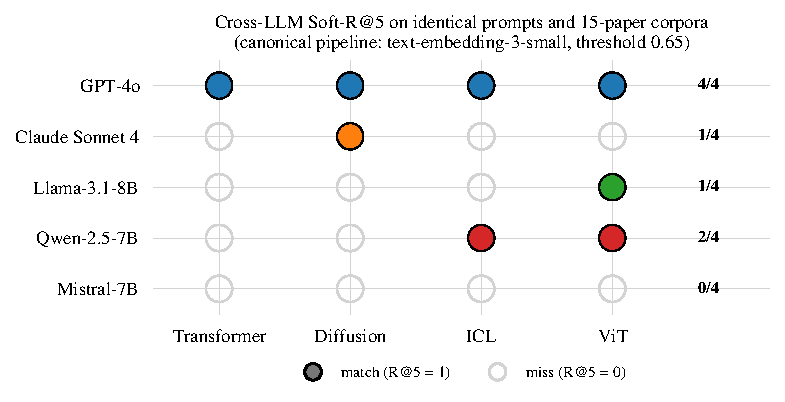
\includegraphics[width=\columnwidth]{figs/fig_cross_llm_bar.pdf}
\caption{Cross-LLM Soft-R@5 per primary paradigm, canonical pipeline (text-embedding-3-small, threshold 0.65). The 5-model spread (GPT-4o 4/4 down to Mistral 0/4) fragments any closed-vs-open framing and exposes model-specific format-compliance interactions with the matcher template.}
\label{fig:crossllm_bar}
\end{figure}

\paragraph{Format-relaxed matcher ablation.}
To test how much of the 5-LLM gap is ranking artifact vs raw extraction recall, we recount each model's primary matches under a relaxed criterion: did \emph{any} of the top-20 confidence-ranked extractions clear the $0.65$ threshold, regardless of confidence rank? Table~\ref{tab:format_relaxed} shows the spread under R@10 (the headline criterion) and under the relaxed any-rank-in-top-20 criterion (\fpath{scripts/run_format_relaxed_matcher.py}).

\begin{table}[h]
\centering
\caption{Format-relaxed matcher ablation. ``Any rank'' = any extraction in top-20-by-confidence clears the 0.65 threshold (regardless of rank). The spread is essentially preserved: Claude gains 1 match (1$\to$2), but GPT-4o stays at 4, Llama at 2, Qwen at 3, Mistral at 0 --- the gap is not primarily a ranking artifact.}
\label{tab:format_relaxed}
\footnotesize
\setlength{\tabcolsep}{4pt}
\begin{tabular}{lccc}
\toprule
Model & R@5 & R@10 & any rank in top-20 \\
\midrule
GPT-4o          & 4 & 4 & 4 \\
Claude Sonnet 4 & 1 & 1 & 2 \\
Llama-3.1-8B    & 1 & 2 & 2 \\
Qwen-2.5-7B     & 2 & 3 & 3 \\
Mistral-7B      & 0 & 0 & 0 \\
\bottomrule
\end{tabular}
\end{table}

The any-rank spread $[4, 2, 2, 3, 0]$ differs from the R@10 spread $[4, 1, 2, 3, 0]$ by exactly one match for Claude only; format-compliance with the matcher template explains \emph{at most one match (Claude)} of the gap. The residual GPT-4o vs Mistral gap (4 vs 0) is in raw extraction recall, not in ranking. The §5.4 ``format-compliance'' framing is therefore a partial explanation; raw capability differences are not excluded.

\section{Prospective Pilot (Exploratory)}\label{app:prospective}

We apply Unbox to 4 current AI paradigms (autoregressive LLMs, RLHF, scaling laws, self-attention). From 12 seed assumptions, 35 hypotheses are generated via TRIZ. Five LLM judge personas evaluate the top 12:

\begin{table}[h]
\centering
\caption{Prospective pilot (5 LLM judge personas, top-12 hypotheses). Moderate inter-judge agreement ($\alpha = 0.34$--$0.47$) reflects legitimate disagreement on creative evaluation; this section is exploratory only.}
\label{tab:prospective}
\footnotesize
\setlength{\tabcolsep}{4pt}
\resizebox{\columnwidth}{!}{%
\begin{tabular}{lcc}
\toprule
Dimension & Avg Score (1--10) & Krippendorff's $\alpha$ \\
\midrule
Novelty & 5.4 & 0.43 \\
Feasibility & 5.9 & 0.34 \\
Impact & 7.0 & 0.37 \\
Clarity & 6.5 & 0.47 \\
\midrule
\textbf{Composite (mean of per-dim avgs)} & \textbf{6.2} (95\% CI: [5.7, 7.0]) & --- \\
\bottomrule
\end{tabular}}
\end{table}

Moderate agreement ($\alpha = 0.34$--$0.47$) reflects legitimate disagreement on creative evaluation. Impact is consistently highest, suggesting hypotheses target important problems. A blinded human expert evaluation remains future work. LLM-as-judge~\cite{zheng2023judging} cannot substitute for expert assessment; this section is exploratory only.

\section{Optional TRIZ-Inspired Diversification (Not Validated)}\label{app:triz}

An early version of this work included a TRIZ-inspired diversification step (\texttt{src/constraint\_breaker.py}) that transforms each extracted assumption through three operators: \textsc{negate}, \textsc{relax}, \textsc{invert}. On the 4 primary shifts with Claude, extraction-only and extraction $+$ TRIZ achieve identical soft-R@10 ($0.75$); on the 4-primary GPT-4o clean-prompt run, the target is already in the top-10 in $4/4$ cases without TRIZ. TRIZ transformations \emph{do} produce near-disjoint hypothesis framings (Jaccard $<0.01$), which may have prospective value, but the prospective pilot (App.~\ref{app:prospective}) is LLM-judge only and inconclusive. We retain the implementation in the supplement for future work but do not include TRIZ in the main pipeline or claim it as a contribution.

\section{Audit-Kit Checklist for LLM-Based Assumption-Recovery Benchmarks}\label{app:checklist}

This checklist formalises the five recommendations of \S\ref{sec:recommendations}. Each item names the confound it isolates, the minimum experimental footprint that exposes it, and the canonical-pipeline parameter set that drives the cost. All five together cost approximately \$15 of API credits on our 4 primary shifts.

\begin{enumerate}[leftmargin=*]
\item \textbf{No-corpus baseline.} Re-run the protocol with only the field name (no paper text). Confound exposed: pretraining memorisation. Minimum footprint: one extraction per paradigm (no corpus). \emph{Decision rule:} if no-corpus R@K $\geq$ with-corpus R@K $-1$, treat the headline as memorisation-dominated.

\item \textbf{Wrong-corpus pairing.} Re-run with a target/corpus mismatch (target field $A$ but corpus from field $B \neq A$). Confound exposed: corpus being ignored when present. Minimum footprint: at least one cross-pair. \emph{Decision rule:} if wrong-corpus R@K $\approx$ with-corpus R@K, the corpus is not causally read; the headline is not a corpus-grounded extraction result.

\item \textbf{Pair-level precision alongside any-of-top-$K$ recall.} Sample $N \geq 50$ stratified (extraction, target)-pair candidates and label each as match / non-match. Confound exposed: the gap between ``$K$th extraction clears threshold'' and ``top extraction matches''. \emph{Decision rule:} report both; recall@$K$ can hit 6/10 from pair-level precision as low as 0.19 (this paper).

\item \textbf{Cross-LLM evaluation (${\geq}2$ models).} Repeat the canonical pipeline with $\geq 2$ architecturally distinct models (e.g.\ closed-API + open-weights, or two different open-weights families). Confound exposed: format compliance vs.\ extraction quality. \emph{Decision rule:} if R@K spreads by ${\geq}2$ across models on identical prompts and corpora, the metric is rewarding format compliance.

\item \textbf{Repeated-run or sensitivity bound.} For closed-model API extractions (which are single-seed by default), report either multi-seed variance (${\geq}3$ seeds) or a temperature / prompt-perturbation sensitivity range. Confound exposed: silent API or prompt drift. \emph{Decision rule:} if the per-seed R@K range exceeds ${\pm}1$ paradigm, treat individual numbers as descriptive of one run, not as a stable point estimate.
\end{enumerate}

\paragraph{Adopting the kit.} The five controls factor: a benchmark author can run them independently as their corpus and compute permit. We release the four scripts (\fpath{scripts/run_no_corpus_control.py}, \fpath{scripts/run_wrong_corpus_control.py}, \fpath{scripts/sample_annotation_pairs.py}, \fpath{scripts/run_multiseed_variance.py}) so adoption is a path edit rather than a re-implementation.

\section{Cross-Embedding Sensitivity}\label{app:crossemb}

The canonical pipeline reports R@$K$ at threshold 0.65 against the \textsc{text-embedding-3-small} embedder. To bound how much of the headline depends on that embedder choice, we re-evaluate the \emph{same} GPT-4o extractions against two alternatives without any new LLM calls: OpenAI \textsc{text-embedding-3-large} and the open-weights \texttt{all-MiniLM-L6-v2} (sentence-transformers). For each embedder we sweep thresholds $\{0.50, 0.55, 0.60, 0.65, 0.70, 0.75\}$ and report the threshold at which primary R@10 saturates.

\begin{table}[h]
\centering
\caption{Cross-embedding sensitivity (re-evaluation of identical GPT-4o extractions). At each embedder's calibrated threshold, primary R@10 stays at $4/4$ and all-paradigm R@10 spans $6$--$8/10$.}
\label{tab:crossemb}
\footnotesize
\setlength{\tabcolsep}{4pt}
\resizebox{\columnwidth}{!}{%
\begin{tabular}{@{}llcc@{}}
\toprule
Embedder & Thr.\ (cal.) & Primary R@10 & All R@10 \\
\midrule
text-embedding-3-small (baseline) & 0.65 & 4/4 & 6/10 \\
text-embedding-3-large            & 0.50 & 4/4 & 8/10 \\
all-MiniLM-L6-v2                  & 0.65 & 4/4 & 7/10 \\
\bottomrule
\end{tabular}}
\end{table}

Two observations:
(i) \textsc{text-embedding-3-large} produces a tighter cosine distribution; at the baseline threshold of 0.65 its primary R@10 drops to $2/4$, but at the F1-calibrated threshold $0.50$ it recovers to $4/4$ and additionally promotes 2 of the previously failing paradigms (all R@10 $= 8/10$).
(ii) \texttt{all-MiniLM-L6-v2} matches the baseline threshold $0.65$ directly and lands at $4/4 / 7/10$ --- the result is therefore not specific to OpenAI embeddings. The qualitative conclusions of \S\ref{sec:main}--\S\ref{sec:diagnostics} (primary $4/4$, no-corpus $4/4$, wrong-corpus $0/4$) are therefore embedder-robust once the threshold is calibrated for each embedder; the embedder-specific 0.65 choice in the main pipeline controls only the absolute all-paradigm count between 6 and 8. Detailed numbers in \fpath{experiments/cross_embedding/summary.json}.

\begin{figure}[h]
\centering
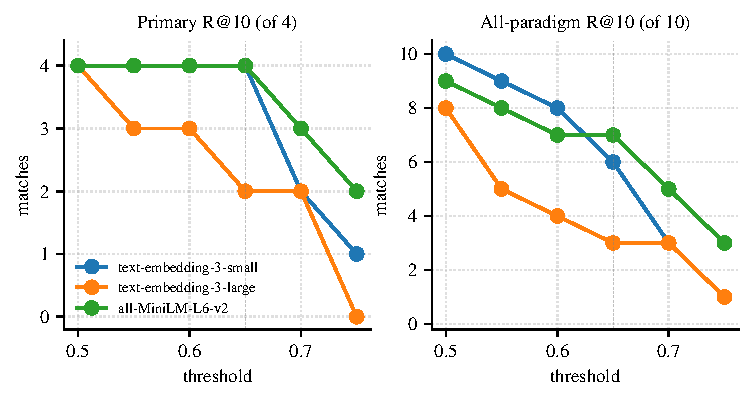
\includegraphics[width=\columnwidth]{figs/fig_threshold.pdf}
\caption{Threshold sweep across 3 embedders. Primary R@10 plateaus at $4/4$ for all three embedders once the threshold is moved off the baseline 0.65 (which is calibrated for \textsc{text-embedding-3-small}); the all-paradigm count varies between 6 and 8 depending on embedder, not the qualitative conclusion.}
\label{fig:threshold_sweep}
\end{figure}

\section{Membership-Inference Cross-Check (Min-K\% Prob)}\label{app:mia}

We test whether a token-level membership-inference attack (MIA) can detect the same contamination that the behavioral no-corpus control surfaces. For each of the 3 OSS models that expose token logprobs (Llama-3.1-8B, Qwen-2.5-7B, Mistral-7B; \fpath{scripts/run_minkpct_mia.py}) we feed every paper in the 4 pre-shift corpora through the model in prefill mode, take the bottom $20\%$ of per-token logprobs, and average them~\cite{shi2024minkpct}. The same statistic is computed on the 45 \emph{synthetic} (definitely non-member) abstracts from \S\ref{sec:memorization} as a baseline.

\begin{table}[h]
\centering
\caption{Min-K\%(20) Prob on the 4 pre-shift corpora (real, $n{=}240$ papers) vs 45 synthetic abstracts (definitely non-member, GPT-generated). Higher (less negative) = more probable = MIA's contamination signal. \emph{Synthetic abstracts are ranked more member-like than real pre-shift papers under all 3 OSS models}; the gap is statistically negative (95\% bootstrap CI strictly below 0) for each model, exposing a stylistic-familiarity confound that defeats the naive MIA reading.}
\label{tab:mia}
\footnotesize
\setlength{\tabcolsep}{4pt}
\resizebox{\columnwidth}{!}{%
\begin{tabular}{@{}lcccc@{}}
\toprule
Model & Real ($n{=}240$) & Synth ($n{=}45$) & Gap & 95\% CI \\
\midrule
Llama-3.1-8B    & $-6.50$ & $-6.02$ & $-0.47$ & $[-0.59, -0.35]$ \\
Qwen-2.5-7B     & $-6.24$ & $-6.00$ & $-0.24$ & $[-0.39, -0.10]$ \\
Mistral-7B      & $-6.10$ & $-5.96$ & $-0.15$ & $[-0.27, -0.02]$ \\
\bottomrule
\end{tabular}}
\end{table}

\begin{figure}[h]
\centering
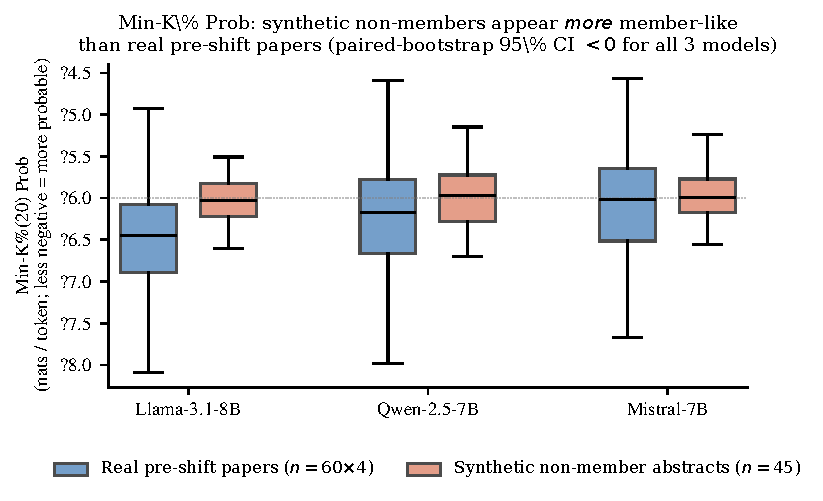
\includegraphics[width=\columnwidth]{figs/fig_mia_box.pdf}
\caption{Per-paper Min-K\%(20) Prob distribution: 240 real pre-shift papers (blue) vs 45 GPT-generated synthetic non-members (orange). In all three OSS models the synthetic non-member distribution sits \emph{above} (less negative than) the real distribution, the opposite of what a naive contamination reading predicts.}
\label{fig:mia_box}
\end{figure}

The gap is \emph{negative} in all 3 models (Figure~\ref{fig:mia_box}): the 45 GPT-generated synthetic abstracts --- guaranteed not in any model's pretraining --- look \emph{more} member-like to Min-K\% Prob than the actual pre-shift corpora do. \emph{Important caveat:} these synthetic abstracts were themselves generated by a GPT-family model and therefore share stylistic distribution with the OSS models' pretraining text far more than pre-2020 archival papers do. The result should be read as a \emph{lower bound on MIA's discriminative power between GPT-style and pre-2020 archival text at this scale}, not as a universal indictment of Min-K\% Prob. With that scope, the finding is still informative: a naive ``Min-K\% high $\Rightarrow$ in training'' reading on this benchmark would mis-call the synthetic non-members as contaminated, while the behavioral no-corpus control --- a uniform $4/4$ recovery on the same 4 paradigms --- gives the direction-correct signal. We view the two modalities as complementary lenses; this paper's empirical observation is that they can disagree at $N=10$ and that the behavioral lens is the one that works here. A non-GPT synth baseline (e.g., generated by Llama itself) would tighten the bound and is left to future work. Detailed numbers in \fpath{experiments/mia_minkpct/}.

\paragraph{Caveat on the synthetic baseline.} The 45 synthetic abstracts were generated by a GPT-family model and therefore share stylistic distribution with the OSS models' pretraining text far more than pre-2020 archival papers do. The negative real-vs-synthetic gap (95\% CI strictly below 0 in all 3 models) is thus an upper bound on MIA's discriminative power between GPT-style and pre-2020 archival text \emph{at this scale}, not a universal claim about MIA; a non-GPT synthetic baseline (e.g., generated by Llama itself) would tighten the bound.

\section{Cross-Domain Applicability of the Audit Kit}\label{app:crossdomain}

The five audit-kit controls (Appendix~\ref{app:checklist}) make no assumption specific to AI/ML literature: they only require (i)~a pre-shift corpus, (ii)~an author- or expert-defined target assumption, and (iii)~a black-box LLM. Direct adaptations to other scientific domains:

\paragraph{Structural biology pre-AlphaFold (2021).} Target assumption: ``Multiple sequence alignment is necessary for accurate protein structure prediction.'' Pre-shift corpus: CASP12--CASP13 method papers ($\leq$2018). The five controls apply unchanged; the no-corpus baseline tests whether ``alignment-based'' patterns are already memorised by frontier LLMs from broader biology literature.

\paragraph{Compressed sensing pre-Donoho/Cand\`es (2006).} Target: ``Nyquist-rate sampling is necessary for exact signal recovery.'' Pre-shift corpus: signal-processing literature $\leq$2005. Wrong-corpus pairing: signal-processing target against information-theory corpus (a tight cross-pair).

\paragraph{NLP pre-Transformer (2017) but \emph{not} pre-BERT.} Target: ``Recurrent connections are necessary for sequence modelling.'' Pre-shift corpus: $\leq$2016 NLP architecture papers (the configuration already used in this paper's main results). This shows the audit kit is self-applicable as a stress test: a benchmark builder can re-run the kit on their own benchmark to detect confounds before reporting headlines.

\paragraph{Note on this paper's footprint.} We do not run the cross-domain demos above; the audit-kit cost (${\sim}\$15$ + 1--2 hours per domain on 4 primary cases) is what we estimate other domains would incur. We list these adaptations to support the ``benchmark-validity probe'' framing in \S\ref{sec:recommendations} and to ground the toolkit's reusability claim.

\section{Failure Mode Taxonomy and Concrete Examples}\label{app:failures}

Each of the 4 R@10 failures (\S\ref{sec:diagnostics} Error analysis) is attributable to a distinct, audit-kit-detectable confound, not to a generic limitation of the protocol. Table~\ref{tab:failure_taxonomy} maps each failure to the kit control that would have surfaced it.

\begin{table}[h]
\centering
\caption{Failure mode taxonomy: each of the 4 R@10 failures has a distinct, kit-detectable root cause.}
\label{tab:failure_taxonomy}
\footnotesize
\setlength{\tabcolsep}{4pt}
\resizebox{\columnwidth}{!}{%
\begin{tabular}{@{}l>{\raggedright\arraybackslash}p{2.4cm}>{\raggedright\arraybackslash}p{3.2cm}@{}}
\toprule
Paradigm & Failure mode & Audit-kit signal \\
\midrule
ResNet    & Coverage gap (target absent in 150 extractions)         & Extraction-keyword check on top-$N$ \\
Word2Vec  & Domain phrasing (``symbolic semantics'')                  & Cross-embedding sensitivity (App.~\ref{app:crossemb}) \\
Dropout   & Implicit assumption (no explicit ``necessary'' frame)     & Threshold sweep / soft-R@10 AUC \\
BERT      & Corpus contamination (OpenAlex retrieved physics paper) & Corpus keyword-precision audit \\
\bottomrule
\end{tabular}}
\end{table}

\paragraph{Concrete failure examples.} For each failure, the top extraction in confidence order and the author-defined target illustrate why semantic similarity drops below threshold:

\begin{itemize}[leftmargin=*,nosep]
\item \textbf{ResNet}. \emph{Target}: ``Deep networks must process information through sequential layers without shortcuts.'' \emph{Top-1 extraction}: ``Convolutional neural networks (CNNs) are essential for extracting powerful features for visual recognition tasks'' (conf = 1.00; best-sim across top-20 = 0.597, below the 0.65 threshold). Cause: the broken assumption (depth-without-shortcuts) is not lexicalised in any pre-2016 paper; the corpus is saturated with CNN-necessity statements.
\item \textbf{Word2Vec}. \emph{Target}: ``Word meaning requires symbolic or hand-crafted feature representations.'' \emph{Top-1}: ``Distributional similarity is necessary for estimating meaning similarity'' (conf = 1.00; best-sim across top-20 = 0.633, below the 0.65 threshold). Pre-shift papers already articulate the distributional alternative as \emph{necessary}; only negation-aware matching would recognise this as expressing the same assumption being broken.
\item \textbf{Dropout}. \emph{Target}: ``All neurons should be active during training for optimal learning.'' \emph{Top-1}: ``Deep neural networks are essential for modern speech recognition systems'' (conf = 0.95; best-sim across top-20 = 0.604, below the 0.65 threshold). The OpenAlex keyword search retrieves application-domain papers rather than papers articulating the all-neurons-active assumption; an explicit ``necessary'' frame for the broken assumption is largely absent from the pre-shift corpus.
\item \textbf{BERT}. \emph{Target}: ``Language model pre-training must be left-to-right (autoregressive).'' \emph{Top-1}: ``Parton distribution functions (PDFs) are essential for predicting outcomes in high-energy particle collisions'' (conf = 1.00; best-sim across top-20 = 0.544, below the 0.65 threshold). Cause: OpenAlex keyword search for ``BERT'' returned a particle-physics paper; this is a corpus-construction artifact rather than an extraction limitation.
\end{itemize}

\section{Multi-Seed Variance}\label{app:multiseed}

\begin{figure}[h]
\centering
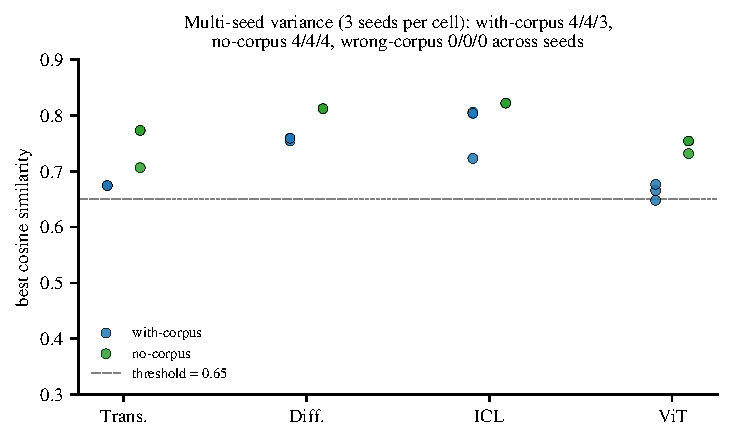
\includegraphics[width=\columnwidth]{figs/fig_multiseed.pdf}
\caption{Per-paradigm best-cosine across 3 seeds (1, 2, 42) for the with-corpus (blue) and no-corpus (green) cells, plus all 4 wrong-corpus pairings (red $\times$). The behavioural conclusions are seed-stable: no-corpus and wrong-corpus cells are identical R@10 across seeds; with-corpus drops the ViT cell of seed 42 just below the dashed 0.65 threshold (the 4/4/3 multi-seed bound in Limitations).}
\label{fig:multiseed}
\end{figure}

\section{Per-Paradigm Rank Heatmap}\label{app:heatmap}

\begin{figure}[!t]
\centering
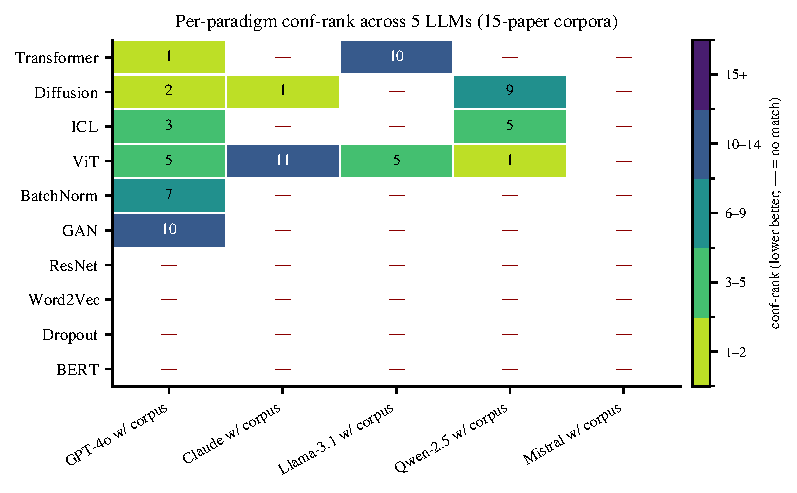
\includegraphics[width=\columnwidth]{figs/fig_rank_heatmap.pdf}
\caption{Confidence rank of the (best-matching) target assumption per paradigm and LLM. Lower = better; ``—'' = no extraction cleared the 0.65 similarity threshold. The matrix makes the per-paradigm spread (6/10 paradigms recovered by GPT-4o, only 1 by Mistral) and the cross-model confound (Diffusion is the only paradigm matched by all five models) directly visible.}
\label{fig:rank_heatmap}
\end{figure}

\pagebreak[4]
\section{Pre-Registered Protocol Snapshot}\label{app:prereg}

The 4-primary-shift protocol was frozen with a SHA-256 hash in \fpath{evidence/protocol_freeze.json} before any extraction was run. The hashed contents (verbatim, anonymised) are:

\begin{samepage}
\begin{lstlisting}[basicstyle=\ttfamily\scriptsize,frame=single]
protocol_id      = "unbox-4primary-v1"
paradigms        = ["transformer","diffusion","icl","vit"]
year_guards      = {transformer:<=2016, diffusion:<=2019,
                    icl:<=2019, vit:<=2019}
target_assumptions = (author-defined; aliases 2--3 per paradigm,
                      stored in data/paradigm_shift_mapping.json)
soft_match       = "cosine >= 0.65 vs any alias"
embedding_model  = "text-embedding-3-small"
primary_metric   = "Soft-Recall@K for K in {5,10,20}"
extraction_model = "Claude Sonnet 4" (initial), "GPT-4o" (canonical)
prompt_variant   = "field-wide paradigmatic" (clean, no few-shot)
papers_per_paradigm = 15 (canonical) / 60 (extended)
seed             = 42 ; temperature = 0
\end{lstlisting}
\end{samepage}

Everything outside this snapshot --- the 6-case extension, retrieval baselines, contamination diagnostics, calibration, error analysis, synthetic/niche controls, cross-LLM sweep, cross-embedding probe, MIA cross-check, multi-seed variance, wrong-corpus pairings (4 and 12), and the audit-kit recommendations --- is \emph{post-hoc}. We label every such result transparently as a stress test or extension in its respective section.

\section{What We Tried and Dropped}\label{app:dropped}

\paragraph{Similarity-reranked output.} An earlier pipeline (\fpath{experiments/gpt4o_clean_prompt/summary_STALE_similarity_reranked.json}) re-sorted extractions by cosine similarity to the target instead of by extraction confidence. This inflates R@K by construction (the highest-similarity extraction is always at rank 1 by definition) and we therefore quarantined it; the canonical pipeline uses confidence ordering only.

\paragraph{TRIZ-inspired diversification.} Section~\ref{app:triz} describes the TRIZ pipeline (negate / relax / invert). It produced near-disjoint hypothesis framings but did not improve retrospective recall (extraction-only and extraction+TRIZ both achieve 0.75 R@10 on the 4 primary shifts with Claude). We retained the implementation but dropped TRIZ from the main pipeline.

\paragraph{Early no-corpus prompt variant.} An initial no-corpus probe handed the model the field name plus the publication year (e.g.\ ``Transformer (2017)''). This leaked the breakthrough date and inflated no-corpus recall above the corpus-grounded baseline. We replaced it with the field-name-only variant used throughout the paper (\fpath{scripts/run_no_corpus_control.py}, \texttt{FIELD\_NAMES\_NO\_YEAR}); both variants are released in the artefact for transparency.

\paragraph{Rule-based 80-pair simulation as ``human'' agreement.} Earlier versions reported $\kappa = 0.97$ from two deterministic keyword-pattern labelers (\fpath{scripts/run_rulebased_match_simulation.py}) as a human-annotation result. This was a simulation, not human annotation, and is now reported as such in \S\ref{sec:diagnostics} and Appendix~\ref{app:sensitivity}; the 10-rater human study (\S\ref{sec:diagnostics}, $\kappa = 0.70$) supersedes it.

\section{Reproduction Walkthrough}\label{app:repro}

The single command \texttt{make reproduce-tables} runs \fpath{scripts/reproduce_paper_tables.py}, which performs 73 offline assertions against the frozen JSON artefacts (no API calls). Categories and counts:

\begin{itemize}[leftmargin=*,nosep]
\item \emph{Table~\ref{tab:results}} main 10-case (32 assertions: 10 paradigms $\times$ 3 metrics + 2 aggregate)
\item \emph{TF-IDF / BM25 retrieval baselines} (2)
\item \emph{Contamination Spearman correlations} (2)
\item \emph{Calibration: gap 0.025, monotonicity 10/10} (2)
\item \emph{Error analysis: ResNet 0/150, BERT keywords absent} (2)
\item \emph{Synthetic 3 fields with rank 1 / 2 / 32} (1)
\item \emph{Wrong-corpus 4 pairings 0/4 and 12 pairings 0/12} (6)
\item \emph{Synthetic Scenario-2 with-corpus rank 2 vs no-corpus 27} (2)
\item \emph{Cross-LLM primary R@5 per model (5 sources)} (5)
\item \emph{Niche subfield 1/8 with-corpus, 2/7 no-corpus} (2)
\item \emph{Human validation: $\alpha{=}0.634$, $\kappa{=}0.702$, AC 79/80} (4)
\item \emph{Cross-embedding primary R@10 4/4 at calibrated threshold} (4)
\item \emph{Min-K\% real-synth gap negative + 95\% CI strict-negative per model} (6)
\item \emph{Multi-seed variance per-seed R@10} (3)
\end{itemize}

The full breakdown is in \fpath{scripts/reproduce_paper_tables.py}; each \texttt{check()} call corresponds to one assertion. If any number in the paper is wrong relative to the stored artefact the script prints which value is expected vs.\ what was found and exits non-zero. A new contributor can therefore verify the paper's full numerical content in seconds against the supplement.

\section{Rater Demographics}\label{app:raters}

The 10-rater human validation panel (R01--R10; raw identities withheld) was drawn from the authors' professional network. Self-reported ML experience distribution at the time of the rating task (anonymous Likert form, no IRB-grade survey instrument): \emph{${\geq}5$ years} (3 raters), \emph{2--5 years} (5 raters), \emph{1--2 years} (2 raters). All raters held at least a bachelor's degree in a computational field and reported familiarity with the ``X is necessary for Y'' assumption-recovery format used in the rating instrument. No personally identifying information beyond R01--R10 mappings is released; the raw rater CSVs are deliberately not included in the supplement (only the anonymised aggregate \fpath{annotation/g1_results.json} is). Participation was voluntary with a small honorarium or acknowledgment offered.

\end{document}
